\documentclass{beamer}

\input{preamble.tex}
\usepackage{breqn} % Breaks lines

\usepackage{amsmath}
\usepackage{mathtools}

\usepackage{pdfpages} % \includepdf

\usepackage{listings} % R code
\usepackage{verbatim} % verbatim

% packages for bibs and cites
% \usepackage{natbib}
% \usepackage{har2nat}
% \newcommand{\possessivecite}[1]{\citeauthor{#1}'s \citeyearpar{#1}}
% \usepackage{breakcites}
% \usepackage{alltt}

% Setup math operators
\DeclareMathOperator{\E}{E} \DeclareMathOperator{\tr}{tr} \DeclareMathOperator{\se}{se} \DeclareMathOperator{\I}{I} \DeclareMathOperator{\sign}{sign} \DeclareMathOperator{\supp}{supp} \DeclareMathOperator{\plim}{plim}
\DeclareMathOperator*{\dlim}{\mathnormal{d}\mkern2mu-lim}
\newcommand\independent{\protect\mathpalette{\protect\independenT}{\perp}}
   \def\independenT#1#2{\mathrel{\rlap{$#1#2$}\mkern2mu{#1#2}}}
\newcommand*\colvec[1]{\begin{pmatrix}#1\end{pmatrix}}

\newcommand{\myurlshort}[2]{\href{#1}{\textcolor{gray}{\textsf{#2}}}}


\begin{document}

\imageframe{./lecture_includes/cover.png}


% ---- Content ----

   

\section{Introduction to course}

\subsection{What is Mixtape Sessions?}


\begin{frame}{Welcome!}

  \begin{itemize}
	\item I'm Scott Cunningham, professor of economics at Baylor University, author of \underline{Causal Inference: the Mixtape}
	\item I teach and host workshops on causal inference all over the world because I believe many people do not have all the opportunities they want to have that they believe will help them be successful in their research and careers 
	\item Workshops can be helpful ways to continue our education in methods that are otherwise inaccessible for whatever reason
		\begin{itemize}
	\item Previous speakers include Alberto Abadie (MIT), Peter Hull (Brown), Jon Roth (Brown), Rocio Titunik (Princeton), Brigham Frandsen (BYU), Brantly Callaway (UGA), Jeff Gortmaker and Ariel Pakes (Harvard)
  \end{itemize}
  \end{itemize}

\end{frame}



\begin{frame}{What is Mixtape Sessions?}

  \begin{itemize}
    \item Mixtape Sessions is my online platform started in November 2021 to ``democratize causal inference'' by helping connect people, from beginner to advanced, with material and teachers that for various reasons may not be accessible otherwise
    \item I tend to emphasize intuition, mechanics, narrow calculations, meaning, assumptions, code including actually taking time to code, advocate for data visualization -- in other words the art and the science
    \item I decided to start teaching a workshop on synthetic control given it is considered one of the more important innovations in causal inference of the last twenty years (Athey and Imbens 2017)
  \end{itemize}

\end{frame}

\begin{frame}{2-day Causal Inference Workshop}

  \begin{itemize}
    \item We workshop together for 2-days, 9am to 5pm CST with 15 min breaks on the hour and a 1-hour lunch break at noon CST
    \item I mix exposition, discussion of papers, coding exercises and discussion as best as I can
    \item I see this workshop as attempting to explain the method, explain some papers, but mainly towards providing guidance on projects using synthetic control, not simply the abstractions of the method 
  \end{itemize}

\end{frame}

\begin{frame}{What my pedagogy is like}

\begin{itemize}
\item Long days that don't feel long because it's high energy, with regular breaks including lunch
\item Move between the econometrics, applications, code, spreadsheets, exercises
\item Ask questions at any point; I'll do my best to answer them and if I can't Kyle can
\end{itemize}

\end{frame}



\begin{frame}{Class goals}

  \begin{enumerate}
    \item \textbf{Confidence}: You will feel like you have a good understanding of synthetic control so that by the end it doesn't feel all that mysterious or intimidating
    \item \textbf{Comprehension}: You will have learned a lot both conceptually and in the specifics, particularly with regards to issues around identification and estimation
    \item \textbf{Competency}: You will have more knowledge of programming syntax in Stata and R (and python!) so that later you can apply this in your own work
  \end{enumerate}

\end{frame}


%\begin{frame}{Causal Inference table of contents}
%  \centering
%  \includegraphics[scale=0.5,height=6.5cm, width=10cm]{./lecture_includes/part1}
%\end{frame}

%\begin{frame}{Causal Inference Part 2}
%  \centering
%  \includegraphics[scale=0.5,height=6.5cm, width=10cm]{./lecture_includes/part2}
%  \url{https://www.mixtapesessions.io/session/ci_II_aug20}
%\end{frame}




\begin{frame}{Github repo}

  \begin{itemize}
    \item We will communicate with one another regularly in the Discord channel and I will always be monitoring it
    \item Encourage you to talk to each other there, help one another, network with one another, coauthor with one another!
    \item I will be distributing things to you, like code and slides, via the github repo: \url{https://github.com/Mixtape-Sessions/Causal-Inference-3.git}
    \item Each lecture will be recorded and then uploaded to Vimeo as a password protected file that you'll have access to into perpetuity
    \item Kyle Butts and I are committed to over time making the Github Repository like an open public library where the only club goods are (a) recordings, (b) Discord and (c) live lectures
  \end{itemize}

\end{frame}

\begin{frame}{Topics}

  \begin{enumerate}
    \item Synthetic control traditionally without extrapolation
    \item Synthetic control with extrapolation and bias adjustment
    \item Aggregating across outcomes and noisy time series
    \item Revisiting the event study from finance
    \item Multiple treated units, staggered adoption, and synthetic diff-in-diff
  \end{enumerate}

\end{frame}

\subsection{Potential outcomes review}

\begin{frame}{Causal Inference vs Prediction}
  \centering
  \includegraphics[scale=0.5,height=6.5cm, width=10cm]{./lecture_includes/prediction_causality.png}
\end{frame}

\begin{frame}{Causal Inference vs Prediction}

  \begin{columns}
    \column{0.48\linewidth}
    \centering
    \textbf{Traditional prediction}
    \begin{itemize}
      \item Traditional prediction seeks to detect patterns in data and fit functional relationships between variables with a high degree of accuracy
      \item ``Does this person have heart disease?'', ``How many books will I sell?''
      \item It is not predictions of what effect a choice will have, though
    \end{itemize}
    \column{0.48\linewidth}
    \centering
    \textbf{Causal inference}
    \begin{itemize}
      \item Causal inference is also a type of prediction, but it's a prediction of a \emph{counterfactual} associated with a particular \emph{choice taken}
      \item Causal inference takes that predicted (or imputed) counterfactual and constructs a causal effect that we hope tells us about a future in the event of a similar choice taken
    \end{itemize}
  \end{columns}
\end{frame}





\begin{frame}
\frametitle{Warranted Belief and Causal Inference}
\begin{itemize}
  \item The goal in causal inference is  \emph{psychological}
  \item When is a correlation \emph{credibly} a causal effect?
  \item When is it a "warranted belief" to believe that one thing caused another when observed in quantitative data and analyzed with statistics?
\end{itemize}
\end{frame}


\begin{frame}
\frametitle{RCT as Thought Experiment}
\begin{itemize}
\item It's helpful to start every project using the randomized controlled trial (RCT) as a thought experiment
	\begin{itemize}
	\item Ask yourself if you had a million dollars and complete freedom, what \emph{randomized} experiment would you run?
	\item It helps you separate out pure description and pure prediction from causal identification
	\item If you cannot articulate the randomization of something to a group of people, pause and start over
	\end{itemize}
\end{itemize}

\end{frame}

\begin{frame}{Decomposition Formula}

\begin{itemize}
\item If we compare the average outcome measured for different two groups -- one treated, one not treated -- then that "simple difference in mean outcomes" (SDO) is \textbf{always equal to}:

\begin{eqnarray*}
SDO &=& \texttt{Average causal effect}  \\
&&+ \texttt{Selection Bias} \\
&&+ \texttt{Heterogenous Treatment Effect Bias}
\end{eqnarray*}
\item Selection bias means the two groups were always going to have different outcomes even if they hadn't been treated
\item Heterogenous treatment effect bias means the two groups were also different with respect to their response to the treatment
\end{itemize}

\end{frame}

\begin{frame}
\frametitle{Decomposition Formula}

\begin{itemize}
\item The decomposition formula is an identity, not a theorem -- it is in other words \textbf{always true}
\item One of the unique features of randomization is that since it is a data generating process independent of the features of the data, it makes the the treatment and control group equal in large samples on all things
\item That is, equal \textbf{except for the fact} that one group was treated and one wasn't
\item This "equivalence in expectation" deletes selection bias and heterogenous treatment effect bias leaving only the first term -- the average effect of the treatment
\end{itemize}

\end{frame}

\begin{frame}
\frametitle{RCT Framing Synthetic Control}
\begin{itemize}
\item In many industry and policy applications, you simply cannot run the RCT you want
	\begin{itemize}
	\item Maybe Uber wants to know the effect of some new self-driving program, but doesn't want to randomize it
	\item It decides to roll it out in Austin, Texas only
	\item Who is the control group?  How will they be chosen?
	\end{itemize}
  \item Synthetic control methods are usually candidates for causal inference in these situations because they work well with quasi-experimental policies at aggregate levels
  \item They also use data driven procedures to find optimal comparison groups
\end{itemize}
\end{frame}






\begin{frame}{Potential outcomes history}

\begin{itemize}

\item Causality (metaphysics and philosophy) versus causal inference (epistemology and psychology)
\item Should I believe that this one thing caused another thing -- it's about credibility, evidence and beliefs
\item We'll introduce briefly the notation we use throughout called potential outcomes which is a language rooted in a 1923 thesis by Jerzy Neyman, philosophical positions by JS Mill in the 1800s, and modern research agenda by Don Rubin
\item Throughout the workshop, we will be focused on \textbf{binary treatment variables} applied to large populations
\end{itemize}

\end{frame}




\begin{frame}{Potential outcomes notation}
	
	\begin{itemize}
	\item Let the treatment be a binary variable: $$D_{i,t} =\begin{cases} 1 \text{ if exposed to autonomous vehicle fleet at time $t$} \\ 0 \text{ if not exposed to autonomous vehicle fleet at time $t$} \end{cases}$$where $i$ indexes an individual observation, such as a person, though for our workshop it'll be an aggregate region

	\end{itemize}
\end{frame}

\begin{frame}{Potential outcomes notation}
	
	\begin{itemize}

	\item Potential outcomes: $$Y_{i,t}^j =\begin{cases} 1 \text{: accidents at time $t$ if self-driving vehicles} \\ 0 \text{: accidents at time $t$ if no self-driving vehicles} \end{cases}$$where $j$ indexes a hypothetical state of the world 

	\end{itemize}
\end{frame}



\begin{frame}{Treatment effect definitions}


	\begin{block}{Individual treatment effect}
	    The individual treatment effect,  $\delta_i$, equals $Y_i^1-Y_i^0$
	\end{block}
Measures the effect of self-driving vehicles on accidents at the unit level. 

\bigskip

Causal inference is a missing data problem in that no one knows the counterfactual because it is "missing" 

\bigskip

Though here it is more "fictional" than simply "missing" as these missing data \textbf{do not exist anywhere}

	
\end{frame}


\begin{frame}{Conditional Average Treatment Effects}	
	\begin{block}{Average Treatment Effect on the Treated (ATT)}
	The average treatment effect on the treatment group is equal to the average treatment effect conditional on being a treatment group member:
		\begin{eqnarray*}
		E[\delta|D=1]&=&E[Y^1-Y^0|D=1] \nonumber \\
		&=&E[Y^1|D=1]-\textcolor{red}{E[Y^0|D=1]}
		\end{eqnarray*}
	\end{block}
	
	\bigskip

Example: The ATT is the averaging of the city's treatment effects who got the policy and it is the \textbf{only} causal effect both synthetic control \emph{and} difference-in-differences can estimate
	
\end{frame}




\section{Original synthetic control method}


\begin{frame}[plain]
	\begin{figure}
	\includegraphics[scale=0.25]{./lecture_includes/currie_synth.png}
	\end{figure}
\end{frame}

	
\begin{frame}{What is a comparative case study?}

\begin{itemize}
\item Originally designed for comparative case studies, but now can accomodate multiple treated units, differential timing, bias adjustment, modifications to difference-in-differences
\item Comparative case studies compare a single aggregate unit (like a country) to another unit (like another country) to make statements about causal effects from aggregate policies or events
\item But the single treated unit can be any aggregate unit: a country, a state, school, firm, etc. 
\end{itemize}

\end{frame}

\begin{frame}{What is a comparative case study?}

 Social scientists traditionally approached comparative case studies in one of two ways:

	\begin{enumerate}
	\item \textcolor{blue}{Qualitatively} (political science)
	\item \textcolor{red}{Quantitatively} (economics)
	\end{enumerate}

\end{frame}



\begin{frame}{First synthetic control paper}

 
``The Economic Costs of Conflict: A Case Study of Basque Country'' (2003) by Alberto Abadie and Javier Gardeazabal, \emph{American Economic Review} (see /Readings at Github Repo)

\bigskip
\footnotesize
\begin{quote} ``About synthetic controls: I had played with related notions for some time, thinking about panel data methods to measure the effects of aggregate interventions. But the idea of synthetic controls shaped up in my mind with the Basque Country example. As always, taking vague concepts to data helps. There wasn’t much one could do in terms of DD for the Basque example. When I saw what is now Figure 1 in the Basque paper appearing on my computer screen after the code finished running for the first time, the value of the method became immediately clear.''
\end{quote}


\end{frame}


\begin{frame}{}

\begin{figure}
\includegraphics[scale=0.5]{./lecture_includes/basque_figure1}
\end{figure}

\end{frame}

\begin{frame}{Synth in Abadie's own words}

Approximately 5 minutes

\url{https://youtu.be/19cRm8aKF-I?si=dD13K60RjTt6E4EF&t=265}

\end{frame}



\begin{frame}{\textcolor{blue}{Qualitative} comparative case studies}
	
	\begin{itemize}
	\item In \textcolor{blue}{qualitative} comparative case studies, the goal might be to reason \emph{inductively} the causal effects of events or characteristics of a single unit on some outcome, oftentimes through logic and historical analysis.  
		\begin{itemize}
		\item Classic example of comparative case study approach is Alexis de Toqueville's \underline{Democracy in America} (but he is regularly comparing the US to France)
		\end{itemize}
	\item Sometimes there may not be an explicit counterfactual, or if there is, it's not principled (subjective researcher decision)
	\item Quantitative claims about causal effects are unlikely -- de Toqueville's won't claim GDP per capita fell \$500 when compared against France
	\end{itemize}
\end{frame}

\begin{frame}{Traditional \textcolor{red}{quantitative} comparative case studies}

\begin{itemize}
	\item Traditional  \textcolor{red}{quantitative}  comparative case studies are explicitly causal designs in that there is a treatment and control, usually involving natural experiment on a single aggregate unit
	\item Comparison focuses on the the evolution of an aggregate outcome for the unit affected by the intervention to the evolution of the same \emph{ad hoc} aggregate control group (Card 1990; Card and Krueger 1994)
	\item It'll essentially be diff-in-diff, but it may not use the event study, and the point is the choice of controls is a subset of all possible controls
\end{itemize}

\end{frame}

\begin{frame}{Pros of the traditional comparative case study}
	Pros:

		\begin{itemize}
		\item Takes advantage of policy interventions that take place at an aggregate level (which is common and so this is useful)
		\item Aggregate/macro data are often available (which may be all we have)
		\end{itemize}
\end{frame}

\begin{frame}{Cons of the traditional comparative case study}
	Cons:

		\begin{itemize}
		\item Selection of control group is \emph{ad hoc} -- opens up researcher biases, even unconscious
		\item Standard errors do not reflect uncertainty about the ability of the control group to reproduce the counterfactual of interest
		\end{itemize}
\end{frame}


\begin{frame}{Description of the Mariel Boatlift}
	
	\begin{itemize}
	\item In 1980, Fidel Castro allowed anyone to leave Cuba so long as they did in the fall from the Mariel boat dock.
	\item The Mariel Boatlift brought 100,000 Cubans to Miami which increased the Miami labor force by 7\%
	\item Card (1990) uses the Mariel Boatlift as a natural experiment to measure the effect of a sudden influx of immigrants on unemployment among less-skilled natives
	\item His question was how do inflows of immigrants affect the wages and employment of natives in local US labor markets?
	\item Individual-level data on unemployment from the Current Population Survey (CPS) for Miami and comparison cities
	\end{itemize}
\end{frame}


\begin{frame}[plain]
	\begin{figure}
	\includegraphics[scale=0.25]{./lecture_includes/boatlift2.png}
	\end{figure}
\end{frame}

\begin{frame}[plain]
	\begin{figure}
	\includegraphics[scale=0.25]{./lecture_includes/boatlift3.png}
	\end{figure}
\end{frame}

\begin{frame}[plain]
	\begin{figure}
	\includegraphics[scale=0.25]{./lecture_includes/boatlift4.png}
	\end{figure}
\end{frame}



\begin{frame}{Selecting control groups}

\begin{itemize}

\item His treatment group was low skill workers in Miami since that's where Cubans went
\item But which control group?
\item He chose Atlanta, Los Angeles, Houston, Tampa-St. Petersburg

\end{itemize}

\end{frame}



\begin{frame}{Why these four?}

	\begin{figure}
	\includegraphics[scale=0.25]{./lecture_includes/card_illr.png}
	\end{figure}

\end{frame}

\begin{frame}{Diff-in-diff}
	
	\begin{figure}
	\includegraphics[scale=0.75]{./lecture_includes/abadie_2.pdf}
	\end{figure}
\end{frame}

\begin{frame}{Parallel trends}

\begin{itemize}
\item Card's analysis used diff-in-diff to estimate the impact of the Mariel boatlift on domestic labor markets
\item His estimate is unbiased if $\Delta E[Y^0]$ for the comparison cities approximates the counterfactual $\textcolor{violet-red}{\Delta E[Y^0]}$ for the treatment group
\item Card selected his controls based on a mixture of matching logic (e.g., covariates) and trend logic (e.g., employment growth) but does not report much
\item Black result would have been positive, too, were it not that the comparison cities growth was twice as large
\item Creates uncertainty about his null result -- was it no effect or was it the control group?
\end{itemize}

\end{frame}


\begin{frame}{Synthetic Control}
	
	\begin{itemize}
	\item Abadie and Gardeazabal (2003) introduced synthetic control in the AER in a study of a terrorist attack in Spain (Basque Country) on GDP
	\item Revisited again in a 2010 JASA with Diamond and Hainmueller, two political scientists who were PhD students at Harvard (more proofs and inference)
	\item Basic idea is to use a combination of comparison units as counterfactual for a treated unit where the units are chosen according to a data driven procedure
	\end{itemize}
\end{frame}


\begin{frame}{Researcher's objectives}

\begin{itemize}
	\item Simple terms: Find a weighted average of donor pool units that "look like" the treatment group before the treatment happened \emph{on outcomes}
	\item More technical way of saying it:
		\begin{itemize}
		\item Synthetic control is a constrained minimization problem where the target goal is the minimization of a vector of squared gaps in pre-treatment characteristics
	\item Choice vector is an endogenous weights that are constant per control group unit over time and range from [0,1). 
	\item Our goal here is to reproduce the counterfactual of a treated unit by finding the combination of untreated units that best resembles the treated unit \emph{before} the intervention in terms of the values of $k$ relevant covariates (predictors of the outcome of interest)
		\end{itemize}
	\item Method selects \emph{weighted average of all potential comparison units} that best resembles the characteristics of the treated unit(s) - called the ``synthetic control''
\end{itemize}

\end{frame}



\begin{frame}{Synthetic control method: advantages}
	
	\begin{itemize}
	\item ``Convex hull'' means synth is a non-negatively weighted average of donor pool units that on closely resemble the treatment group over time.
	\item Constraints on the model use non-negative weights which does not allow for extrapolation 
	\item Makes explicit the contribution of each comparison unit to the counterfactual 
	\item Formalizing the way comparison units are chosen has direct implications for inference
	\end{itemize}
\end{frame}




\begin{frame}{Notation and setup}
	
Suppose that we observe $J+1$ units in periods $1, 2, \dots, T$
		\begin{itemize}
		\item Unit ``one'' is exposed to the intervention of interest (that is, ``treated'') during periods $T_0+1, \dots, T$
		\item The remaining $J$ are an untreated reservoir of potential controls (a ``donor pool'')
		\end{itemize}	
\end{frame}


\begin{frame}{Potential outcomes notation}

		\begin{itemize}
		\item Let $Y_{it}^0$ be the outcome that would be observed for unit $i$ at time $t$ in the absence of the intervention
		\item Let $Y_{it}^1$ be the outcome that would be observed for unit $i$ at time $t$ if unit $i$ is exposed to the intervention in periods $T_0+1$ to $T$.
		\end{itemize}

\end{frame}

\begin{frame}{Group-time ATT with only one treated group}

Treatment effect parameter is defined as dynamic ATT where 

\begin{eqnarray*}
\delta_{1t}&=&Y_{1t}^1 - Y_{1t}^0 \\
&=& Y_{1t} - Y_{1t}^0 
\end{eqnarray*} for each post-treatment period, $t>T_0$ and $Y_{1t}$ is the outcome for unit one at time $t$. We will estimate $Y^0_{1t}$ using the $J$ units in the donor pool 

\end{frame}

\begin{frame}{Optimal weights}
	
	\begin{itemize}
	\item Let $W=(w_2, \dots, w_{J+1})'$ with $w_j\geq 0$ for $j=2, \dots, J+1$ and $w_2+\dots+w_{j+1}=1$. Each value of $W$ represents a potential synthetic control
	\item Let $X_1$ be a $(k\times 1)$ vector of pre-intervention characteristics for the treated unit.  Similarly, let $X_0$ be a $(k\times J)$ matrix which contains the same variables for the unaffected units.
	\item The vector $W^*=(w_2^*, \dots, w_{J+1}^*)'$ is chosen to minimize $||X_1-X_0W||$, subject to our weight constraints
	\end{itemize}
\end{frame}

\begin{frame}{Optimal weights differ by another weighting matrix}
	
Abadie, et al. consider $$||X_1 - X_0W||=\sqrt{(X_1-X_0W)'V(X_1-X_0W)}$$where $X_{jm}$ is the value of the $m$-th covariates for unit $j$ and $V$ is some $(k\times k)$ symmetric and positive semidefinite matrix

\end{frame}

\begin{frame}{Similarity to distance minimization}

\begin{itemize}
\item Bears some resemblance to nearest neighbor matching though I don't want to oversell that
\item There is a unique solution that selects weighting minimizing the distance between the covariates comparison characteristics and treatment group
\item Let's look at an example from nearest neighbor matching of minimizing Euclidean distance to help firm the ideas
\item \url{https://docs.google.com/spreadsheets/d/1iro1Qzrr1eLDY_LJVzOYvnQZWmxY8JyTcDf6YcdhkwQ/edit?usp=sharing}
\end{itemize}

\end{frame}

\begin{frame}{Illustration of the "optimal weight"}

\begin{figure}
\includegraphics[scale=0.25]{./lecture_includes/synth_optimal_weight}
\end{figure}

\end{frame}



\begin{frame}{More on the V matrix}

Typically, $V$ is diagonal with main diagonal $v_1, \dots, v_k$.  Then, the synthetic control weights $w_2^*, \dots, w_{J+1}^*$ minimize: $$\sum_{m=1}^k v_m \bigg(X_{1m} - \sum_{j=2}^{J+1}w_jX_{jm}\bigg)^2$$ where $v_m$ is a weight that reflects the relative importance that we assign to the $m$-th variable when we measure the discrepancy between the treated unit and the synthetic controls

\end{frame}

\begin{frame}{Choice of $V$ is critical}
	
		\begin{itemize}
		\item The synthetic control $W^*(V^*)$ is meant to reproduce the behavior of the outcome variable for the treated unit in the absence of the treatment
		\item Therefore, the $V^*$ weights directly shape $W^*$
		\end{itemize}
\end{frame}

\begin{frame}{Estimating the $V$ matrix}
	
 Choice of $v_1, \dots, v_k$ can be based on
		\begin{itemize}
		\item Assess the predictive power of the covariates using regression
		\item Subjectively assess the predictive power of each of the covariates, or calibration inspecting how different values for $v_1, \dots, v_k$ affect the discrepancies between the treated unit and the synthetic control
		\item Minimize mean square prediction error (MSPE) for the pre-treatment period (default):
			\begin{eqnarray*}
			\sum_{t=1}^{T_0} \bigg(Y_{1t} - \sum_{j=2}^J w_j^*(V^*)Y_{jt} \bigg)^2
			\end{eqnarray*}
		\end{itemize}
\end{frame}

\begin{frame}{Cross validation}

\begin{itemize}
		\item Abadie recommends cross validation for selecting the covariates
		\item Divide the pre-treatment period into an initial \textbf{training} period and a subsequent \textbf{validation} period
		\item For any given $V$, calculate $W^*(V)$ in the training period.
		\item Minimize the MSPE of $W^*(V)$ in the validation period
\end{itemize}

\bigskip

Let's look at an example from the 2010 JASA paper with Hainmueller and Diamond

\end{frame}


\begin{frame}{Example: California's Proposition 99}
	
	\begin{itemize}
	\item In 1988, California first passed comprehensive tobacco control legislation:
		\begin{itemize}
		\item increased cigarette tax by 25 cents/pack
		\item earmarked tax revenues to health and anti-smoking budgets
		\item funded anti-smoking media campaigns
		\item spurred clean-air ordinances throughout the state
		\item produced more than \$100 million per year in anti-tobacco projects
		\end{itemize}
	\item Other states that subsequently passed control programs are excluded from donor pool of controls (AK, AZ, FL, HI, MA, MD, MI, NJ, OR, WA, DC)
	\end{itemize}
\end{frame}

\begin{frame}{Cigarette Consumption: CA and the Rest of the US}
	
	\begin{figure}
	\includegraphics[scale=0.75]{./lecture_includes/abadie_3.pdf}
	\end{figure}
\end{frame}

\begin{frame}{Cigarette Consumption: CA and synthetic CA}
	
	\begin{figure}
	\includegraphics[scale=0.75]{./lecture_includes/abadie_4.pdf}
	\end{figure}
\end{frame}

\begin{frame}{Sparsity and Synthetic Control Weights}
	\begin{figure}
	\includegraphics[scale=0.25]{./lecture_includes/synth_smoking_table2.png}
	\end{figure}
\end{frame}



\begin{frame}{Predictor Means: Actual vs. Synthetic California}
	
	\begin{figure}
	\includegraphics[scale=0.75]{./lecture_includes/abadie_5.pdf}
	\end{figure}
\end{frame}

\begin{frame}{Smoking Gap between CA and synthetic CA}
	
	\begin{figure}
	\includegraphics[scale=0.75]{./lecture_includes/abadie_6.pdf}
	\end{figure}
\end{frame}

\begin{frame}{Inference}
	
	\begin{itemize}
	\item To assess significance, we calculate exact p-values under Fisher's sharp null using a test statistic equal to after to before ratio of RMSPE
	\item Exact p-value method
		\begin{itemize}
		\item Iteratively apply the synthetic method to each country/state in the donor pool and obtain a distribution of placebo effects
		\item Compare the gap (RMSPE) for California to the distribution of the placebo gaps. For example the post-Prop. 99 RMSPE is: 
			\begin{eqnarray*}
			RMSPE = \bigg(\frac{1}{T-T_0} \sum_{t=T_0+1}^T \bigg(Y_{1t} - \sum_{j=2}^{J+1} w_j^* Y_{jt}\bigg)^2 \bigg)^{\frac{1}{2}}
			\end{eqnarray*}and the exact p-value is the treatment unit rank divided by $J$
		\end{itemize}
	\end{itemize}
\end{frame}

\begin{frame}{Smoking Gap for CA and 38 control states}
	
	\begin{figure}
	\includegraphics[scale=0.75]{./lecture_includes/abadie_7.pdf}
	\end{figure}
\end{frame}

\begin{frame}{Smoking Gap for CA and 34 control states}
	
	\begin{figure}
	\includegraphics[scale=0.75]{./lecture_includes/abadie_8.pdf}
	\end{figure}
\end{frame}

\begin{frame}{Smoking Gap for CA and 29 control states}
	
	\begin{figure}
	\includegraphics[scale=0.75]{./lecture_includes/abadie_9.pdf}
	\end{figure}
\end{frame}

\begin{frame}{Smoking Gap for CA and 19 control states}
	
	\begin{figure}
	\includegraphics[scale=0.75]{./lecture_includes/abadie_10.pdf}
	\end{figure}
\end{frame}

\begin{frame}{Ratio Post-Prop. 99 RMSPE to Pre-Prop. 99 RMSPE}

	\begin{figure}
	\includegraphics[scale=0.75]{./lecture_includes/abadie_11.pdf}
	\end{figure}
\end{frame}


\begin{frame}{Abadie's Suggestions for Dropping Units from the Donor Pool}
  \begin{itemize}
    \item \textbf{Treated Units:} 
    \begin{itemize}
      \item Drop units exposed to the same or similar intervention.
      \item (e.g., States that passed similar laws during the study period.)
    \end{itemize}
    \item \textbf{Units with Large Idiosyncratic Shocks:}
    \begin{itemize}
      \item Drop units that experienced major unrelated events.
      \item (e.g., Natural disasters, political crises.)
    \end{itemize}
    \item \textbf{Units Very Different in Observables:}
    \begin{itemize}
      \item Drop units very dissimilar in key characteristics to avoid interpolation bias.
      \item (e.g., Comparing a small rural state to a large industrialized one.)
    \end{itemize}
    \item \textbf{Units Affected by Spillovers:}
    \begin{itemize}
      \item Drop units possibly influenced by the treated unit’s intervention.
      \item (e.g., Neighboring regions affected by a tax reform.)
    \end{itemize}
  \end{itemize}
\end{frame}

\begin{frame}{Why Drop Units with Large Idiosyncratic Shocks?}
  \begin{quote}
    ``It is important to eliminate from the donor pool any units that may have suffered large idiosyncratic shocks to the outcome of interest during the study period, if it is judged that such shocks would not have affected the treated unit had it not been treated.'' — Abadie (2021)
  \end{quote}
  \vspace{0.5cm}
  \begin{itemize}
    \item \textbf{Intuition:} We want donor units that show how the treated unit would have evolved without the intervention.
    \item Units hit by unrelated shocks add noise, distort the synthetic control, and are not informative about the treated unit’s natural counterfactual.
  \end{itemize}
\end{frame}

\begin{frame}{Example: Florida and Minimum Wage}
  \begin{itemize}
    \item Study: Impact of New Jersey's minimum wage hike on employment.
    \item Florida (donor unit) experiences a major hurricane during the study window.
    \begin{itemize}
      \item Hurricane tanks employment — unrelated to wage policy.
      \item Florida's employment outcomes diverge from normal labor market trends.
      \item Including Florida would bias the synthetic control downward.
    \end{itemize}
    \item \textbf{Conclusion:} Drop Florida from the donor pool.
  \end{itemize}
\end{frame}

\begin{frame}{Why Large Idiosyncratic Shocks Are Dangerous (1)}
  \begin{itemize}
    \item Synthetic Control assumes donor units are affected only by common latent factors.
    \item A large idiosyncratic shock breaks this assumption — the donor unit evolves for reasons unique to itself.
    \item Weights cannot correct for shocks that are orthogonal to the underlying factor structure.
  \end{itemize}
\end{frame}

\begin{frame}{Why Large Idiosyncratic Shocks Are Dangerous (2)}
  \begin{itemize}
    \item Including shocked units introduces \textbf{irrelevant noise} into the counterfactual.
    \item This noise pulls the synthetic control away from what would have naturally happened to the treated unit.
    \item Better to construct the synthetic control from clean, comparably evolving units.
  \end{itemize}
\end{frame}


\begin{frame}{Sparsity and Weight Distribution}
  \begin{itemize}
    \item \textbf{Sparse Weights Are Typical:}
    \begin{itemize}
      \item Synthetic controls often assign positive weight to only a few donor units.
      \item (e.g., 4 or 5 countries build the synthetic West Germany.)
    \end{itemize}
    \item \textbf{Spread-Out Weights Can Occur:}
    \begin{itemize}
      \item If the treated unit lies inside the donor convex hull, many small positive weights are possible.
      \item (e.g., Each donor unit gets 2–5\% weight instead of a few getting large weights.)
    \end{itemize}
    \item \textbf{Why Prefer Sparsity?}
    \begin{itemize}
      \item Easier interpretation of which units drive the counterfactual.
      \item Allows clear evaluation of potential biases.
    \end{itemize}
  \end{itemize}
\end{frame}


\begin{frame}{Data exercise: Texas Builds Prisons}
	
	\begin{itemize}
	\item The US has the highest prison population of any OECD country in the world 
	\item 2.1 million are currently incarcerated in US federal and state prisons and county jails
	\item Another 4.75 million are on parole
	\item From the early 1970s to the present, incarceration and prison admission rates quintupled in size
	\end{itemize}
\end{frame}



\begin{frame}[plain]

\begin{figure}
\includegraphics[scale=0.5]{./lecture_includes/cook2010.pdf}
\end{figure}
\end{frame}


\begin{frame}{Prison constraints}

	
	\begin{itemize}
	\item Prisons are and have been at capacity for a long time so growth in imprisonment would bite on state corrections
	\item Managing increased flows can only be solved by the following:
		\begin{itemize}
		\item Prison construction
		\item Overcrowding
		\item Paroles
		\end{itemize}
	\item Texas chooses overcrowding
	\end{itemize}
\end{frame}



\begin{frame}{Ruiz v. Estelle 1980}

	
	\begin{itemize}
		\item Class action lawsuit against TX Dept of Corrections (Estelle, warden). 
		\item TDC lost.  Lengthy period of appeals and legal decrees.  
		\item Lengthy period of time relying on paroles to manage flows
	\end{itemize}
\end{frame}

\begin{frame}[plain]
  \includegraphics[scale=0.8]{./lecture_includes/flow_rate_figure.pdf}
\end{frame}

\begin{frame}{Texas prison boom}

Governor Ann Richards (D) 1991-1995
		\begin{itemize}
		\item Operation prison capacity increased 30-35\% in 1993, 1994 and 1995. 
		\item Prison capacity increased from 55,000 in 1992 to 130,000 in 1995.  
		\item Building of new prisons (private and public)
		\end{itemize} 
\end{frame}


\begin{frame}[shrink=30,plain]

\begin{figure}
\includegraphics{./lecture_includes/tdcj.pdf}
\end{figure}
\end{frame}


\begin{frame}[shrink=30,plain]
\begin{figure}
\includegraphics{./lecture_includes/capacity_operational_texas.pdf}
\end{figure}
\end{frame}



\begin{frame}[shrink=30,plain]

\begin{figure}
\includegraphics{./lecture_includes/total_incarceration.pdf}
\end{figure}
\end{frame}

\begin{frame}[shrink=30,plain]

\begin{figure}
\includegraphics{./lecture_includes/synth_placebo_totalincarceration1993.pdf}
\end{figure}
\end{frame}


\begin{frame}{Coding together}

\begin{itemize}
\item Let's go to Mixtape Sessions repository now into /Labs/Texas 
\item I'll walk us through the Stata and R code so you understand the syntax and underlying logic
\item But then I have us a practice assignment 
\end{itemize}

\end{frame}


\begin{frame}{Avoiding Cherry Picking: Subway franchise and Scandal}

	\begin{figure}
	\includegraphics[scale=0.25]{./lecture_includes/subway_8.png}
	\end{figure}

\end{frame}

\begin{frame}{Subway franchise and Scandal}

	\begin{figure}
	\includegraphics[scale=0.25]{./lecture_includes/subway_1.png}
	\end{figure}

\end{frame}


\begin{frame}{Subway franchise and Scandal}

	\begin{figure}
	\includegraphics[scale=0.25]{./lecture_includes/subway_2.png}
	\end{figure}

\end{frame}

\begin{frame}{Subway franchise and Scandal}

	\begin{figure}
	\includegraphics[scale=0.3]{./lecture_includes/subway_3.png}
	\end{figure}

\end{frame}


\begin{frame}{Subway franchise and Scandal}

	\begin{figure}
	\includegraphics[scale=0.3]{./lecture_includes/subway_4.png}
	\end{figure}

\end{frame}

\begin{frame}{Subway franchise and Scandal}

	\begin{figure}
	\includegraphics[scale=0.35]{./lecture_includes/subway_5.png}
	\end{figure}

\end{frame}

\begin{frame}{Subway franchise and Scandal}

	\begin{figure}
	\includegraphics[scale=0.35]{./lecture_includes/subway_6.png}
	\end{figure}

\end{frame}

\begin{frame}{Cherry picking synthetic controls}

\begin{itemize}
\item Abadie, et al. recommended a nested minimization problem using the preintervention data to estimate the SC weights, but very little to no guidance was provided beyond that
\item Historically, a broad range of selection of pre-treatment characteristics were used by early researchers which created researcher degrees of freedom or ``cherry picking synthetic controls''
\item Ferman, Pinto and Possbaum (2020) suggest specific specifications and report all of them with and without covariates
\item Here's an example of the kinds of tables and graphical evidence they suggested researchers follow (followed by what we did)
\end{itemize}

\end{frame}


\begin{frame}{Show p-values across all recommended specifications}

	\begin{figure}
	\includegraphics[scale=0.5]{./lecture_includes/cherry_picking_1.png}
	\end{figure}

\end{frame}

\begin{frame}{Show event study (not placebo) across all recommended specifications}

	\begin{figure}
	\includegraphics[scale=0.5]{./lecture_includes/cherry_picking_2.png}
	\end{figure}

\end{frame}


\begin{frame}{Subway franchise and Scandal}

	\begin{figure}
	\includegraphics[scale=0.25]{./lecture_includes/subway_robustness.png}
	\end{figure}

\end{frame}


\begin{frame}{Subway franchise and Scandal}

	\begin{figure}
	\includegraphics[scale=0.25]{./lecture_includes/subway_7.png}
	\end{figure}

\end{frame}

\begin{frame}{Summarizing}

\begin{itemize}

\item Method is simple: take donor pool units and find a combination of units, weight them, that minimize a distance function subject to two weight constraints $W*$ and $V*$.
\item But what is the bias and what can we do when we think the bias is severe?
\item We now move towards that now by examining the nature of the bias in synthetic control
\end{itemize}

\end{frame}

\section{Imperfect fit}

\subsection{Bounding the bias}

\begin{frame}
\frametitle{Bias of Synthetic Control}

\begin{itemize}
\item Bias in synthetic control comes from failing to match the hidden forces that drive the treated unit's Y(0) potential outcome. 
\item A factor model helps us formalize this idea — if we match well on pre-treatment outcomes, we are indirectly matching on those hidden factors, and the bias becomes small.
\end{itemize}
\end{frame}

\begin{frame}{Suppose $Y^0$ is given by a factor model}


\begin{itemize}
\item What about unmeasured factors affecting the outcome variables as well as heterogeneity in the effect of observed and unobserved factors?

\item Abadie, et al. assume that the missing potential outcome, $Y^0_{it}$, is generated using a factor model

\begin{eqnarray*}
Y_{it}^0 = \alpha_t + \theta_t Z_i + \lambda_t u_i + \varepsilon_{it}
\end{eqnarray*}

%where $\alpha_t$ is an unknown common factor with constant factor loadings across units, and $\lambda_t$ is a vector of unobserved common factors

\end{itemize}

\end{frame}

\begin{frame}{Factor Model Intuition}
  Untreated potential outcomes are given by a factor model:
  \begin{equation}\label{eq:untreated_po}
    Y_{it}^0 = \alpha_t + \theta_t Z_i + \textcolor{navy}{\lambda_t} \textcolor{orange}{u_i} + \varepsilon_{it}
  \end{equation}

  \begin{itemize}
 \item $\alpha_t$ is the time fixed effects, $Z_i$ is observed features, $u_i$ is unobserved features, $\varepsilon_{it}$ is unit-level transitory shock
    \item $\lambda_t$ is the set of \textcolor{navy}{factors} (macroeconomic shock) at time $t$.
    \item $u_i$ is unit $i$'s \textcolor{orange}{factor loading} (exposure) to the shocks.
  \end{itemize}

  For example, $\lambda_t$ is a shock to the returns to technological ability and $u_i$ is unobserved ability.
\end{frame}


\begin{frame}{Factor Model Intuition}
  Untreated potential outcomes are given by a factor model:
  \begin{equation}\label{eq:untreated_po}
    Y_{it}^0 = \alpha_t + \theta_t Z_i + \textcolor{navy}{\lambda_t} \textcolor{orange}{u_i} + \varepsilon_{it}
  \end{equation}


Suppose we found $W^*$ such that:

$$\sum^{J+1}_jw^*_jY_{jt}=Y_{1t}$$ $$\sum^{J+1}_jw^*_jZ_{j}=Z_{1}$$ but realistically only \emph{approximately}

\end{frame}

\begin{frame}{Factor Model Intuition}
  But for the unobserved factors $u_i$, we can only \textbf{hope} that:
  \[
  \sum_{j=2}^{J+1} w_j^* u_j \approx u_1
  \quad \text{(unobserved, approximate matching)}
  \]

  \vspace{0.5cm}

  Since both $\lambda_t' u_i$ (systematic unobserved factors) and $\varepsilon_{it}$ (idiosyncratic shocks) are unobserved, the core challenge is:
  
  \begin{center}
  \textbf{"How can we be sure we are balancing $u_i$ and not simply matching noise $\varepsilon_{it}$?"}
  \end{center}
\end{frame}

\begin{frame}{Thus the Bias Is...}
  \begin{itemize}
    \item So to understand the theoretical source of synthetic control's bias, we write down:
    \[
    \textcolor{red}{Y_{1t}^0} - \sum_{j=2}^{J+1} w_j^* Y_{jt}^0
    \]
    \item Next step:
    \begin{itemize}
      \item Expand both $\textcolor{red}{Y_{1t}^0}$ and $Y_{jt}^0$ using the factor model.
      \item Carefully track what cancels and what remains.
    \end{itemize}
    \item Goal:
    \begin{itemize}
      \item Understand which parts synthetic control matches well, and
      \item Where bias can still enter the estimator.
    \end{itemize}
  \end{itemize}
\end{frame}

\begin{frame}{Expand Both Terms Using the Factor Model}

\begin{eqnarray*}
\underbrace{\textcolor{red}{Y_{1t}^0} - \sum_{j=2}^{J+1} w_j^* Y_{jt}^0}_{\text{bias of synthetic control}} &=& \underbrace{(\alpha_t - \alpha_t)}_{\text{cancels automatically}} \\
&& + \underbrace{(\theta_t Z_1 - \theta_t \sum_j w_j^* Z_j)}_{\text{cancels if observables are matched}} \\
&& + \underbrace{(\lambda_t' u_1 - \lambda_t' \sum_j w_j^* u_j)}_{\text{cancels if unobserved factors are matched}} \\
&& + (\varepsilon_{1t} - \sum_{j=2}^{J+1} w_j^* \varepsilon_{jt})
\end{eqnarray*}
\end{frame}


\begin{frame}{Sources of Synthetic Control Bias}
  After expanding, we see that bias comes from two components:
  \vspace{0.5cm}
  \begin{itemize}
    \item $\lambda_t' (u_1 - \sum_j w_j^* u_j)$
    \begin{itemize}
      \item $\Rightarrow$ Bias from mismatch in \textbf{unobserved factors} 
      \item (e.g., unmeasured policy environment, social norms, culture)
    \end{itemize}
    \item $\varepsilon_{1t} - \sum_j w_j^* \varepsilon_{jt}$
    \begin{itemize}
      \item $\Rightarrow$ Bias from \textbf{idiosyncratic post-treatment shocks}
      \item (e.g., random weather events, isolated firm closures)
    \end{itemize}

  \end{itemize}
 Bias is from mismatch in unobserved factors $u_i$ and residual shocks $\varepsilon_{it}$.
\end{frame}


\begin{frame}{Proxying Unobserved Factors with Pre-Treatment Outcomes}
  \small
  \begin{itemize}
    \item We cannot observe the latent factors $u_i$ directly, but we do observe pre-treatment outcomes (let $s$ be pre-treatment time periods):
    \[
    Y_{is}^0 = \alpha_s + \theta_s Z_i + \lambda_s' u_i + \varepsilon_{is}
    \]
    \item After matching $Z_i$ and cancelling $\alpha_s$, like we showed previously, then variation across $s$ is driven by:
    \[
    \lambda_s' u_i + \varepsilon_{is}
    \]
    \item \textbf{Idea:} Use pre-treatment outcomes to estimate $u_i$ up to noise.
  \end{itemize}
\end{frame}


\begin{frame}{Approximation of SCM Bias}
  \small
  \begin{itemize}
    \item The mismatch in latent factors $\lambda_t' (u_1 - \sum_j w_j^* u_j)$ can be approximated as a weighted sum of pre-treatment residuals:
  \end{itemize}

  \vspace{0.5cm}

  \[
  \sum_{j=2}^{J+1} w_j^* \sum_{s=1}^{T_0} 
  \lambda_t' \left( \sum_{n=1}^{T_0} \lambda_n' \lambda_n \right)^{-1} 
  \lambda_s (\varepsilon_{js} - \varepsilon_{1s})
  \]

  \vspace{0.5cm}

  \begin{itemize}
    \item $\Rightarrow$ Imperfect matching on pre-treatment outcomes shows up as a weighted sum of noise terms.
    \item $\Rightarrow$ With many pre-treatment periods and small $\varepsilon_{it}$, bias shrinks.
  \end{itemize}
\end{frame}





\begin{frame}{When Pre-Treatment Fit is Poor}
  \begin{itemize}
    \item SCM bias is small when the treated unit is well-matched to the synthetic control on pre-treatment outcomes.
    \item But in many real-world settings, \textbf{excellent pre-treatment fit is not possible}.
    \item Then, the SCM estimator can have substantial bias.
    \item \textbf{Idea:} Borrow from bias-corrected matching — adjust for the bias using an outcome model.
  \end{itemize}
\end{frame}

\begin{frame}{Synthetic control bounds}

\begin{itemize}
  \item Abadie, et al. 2010 shows the bounds on the bias and it is based on how closely you're able to fit the synthetic control to the treatment group over time
  \item Bias bound is controlled by a ratio between the scale of the transitory shocks, $\varepsilon_{it}$, and the time length
  \item Your credibility of a synthetic control depends on the extent to which it is able to fit a trajectory  $Y_{1t}$ for an extended pre-intervention period
  \item The idea is that on the shorter series, you're fitting noise ($\varepsilon$) not the factor model
 \end{itemize}
 
 \end{frame}



\begin{frame}{Example of long $T_0$ and transitory shocks}

	\begin{figure}
	\includegraphics[scale=0.25]{./lecture_includes/restud_titlepage}
	\end{figure}

\end{frame}

\begin{frame}{Example of long $T_0$ and transitory shocks}

	\begin{figure}
	\includegraphics[scale=0.20]{./lecture_includes/restud_rapesynth}
	\end{figure}

\end{frame}




\begin{frame}{ Synthetic Control Bias Under Factor Model}
  Synthetic control will do well when you have many time-periods because:
  \begin{enumerate}
    \item You will not fit on the error term $\varepsilon_{it}$ 
    \item Instead, you will find a synthetic control with the same \emph{exposure} to aggregate shocks (matching on factor-loadings)
  \end{enumerate}

  \bigskip
  But what about when we don't have good fit?
\end{frame}

\subsection{Demeaned Synthetic Control}

\begin{frame}{From Abadie, et al. (2010)}

	\begin{figure}
	\includegraphics[scale=0.40]{./lecture_includes/abadie_imperfect_fit}
	\end{figure}

\end{frame}


\begin{frame}{Ferman and Pinto (2021)}

	\begin{figure}
	\includegraphics[scale=0.20]{./lecture_includes/ferman_pinto2021}
	\end{figure}

\end{frame}






\begin{frame}{Imperfect pre-treatment fit }

\begin{itemize}

\item Ferman and Pinto (2021) show that synthetic control will generally be biased if treatment assignment is correlated with an unobserved confounder even in very long pre-treatment periods

\item ``This happens because, in this setting, the SC weights converge to weights that simultaneously attempt to match the factor loadings of the treated unit and to minimize the variance of a linear combination of the idiosyncratic shocks.'' (Ferman and Pinto 2021)

\item So even if you reconstructed the pre-trends with your synth, you may not have recovered the true weights because you'd need a comparison group that was affected by the dynamic confounder in exactly the same way, just not treated

\end{itemize}

\end{frame}


\begin{frame}{Demeaning to address bias}

\begin{itemize}
\item Ferman and Pinto (2021) show that the synthetic control estimator converges to the parameter we want \emph{plus linear} combinations of contemporaneous idiosyncratic shocks and common factors
\item If you assume the idiosyncratic factors cancel out in large samples, then the bias will depend on the differences in how the treated and the synthetic control units are affected by the common shocks
\item They show that it is generally unbiased under the same conditions as diff-in-diff, and can have lower asymptotic variance, but they recommend showing then both diff-in-diff and demeaned synthetic control

\end{itemize}

\end{frame}


\begin{frame}{}

\begin{figure}
\includegraphics[scale=0.25]{./lecture_includes/restud_dd}
\end{figure}

\end{frame}



\begin{frame}{Demeaning to address bias}

\begin{itemize}

\item Cannot compare the original synthetic control with the demeaned synthetic control in terms of bias and variance -- if units with similar factor loadings have similar fixed effects, then matching on levels would be better than demeaning 
\item Demeaning can increase the variance in finite pre-treatment
\item Demeaning also implies extrapolating which is often considered to be one of the hallmark strengths of the original synthetic control estimator -- it does not extrapolate 

\end{itemize}

\end{frame}

\begin{frame}{What did we do?}

\begin{itemize}
\item Our Rhode Island paper began in 2009 and was published in 2018, with working papers in circulation in 2014, well before this imperfect literature
\item One of our main outcomes was reported female rape offenses per 100,000 as measured in the Uniform Crime Reports 
\item Rhode Island is a small state so even relatively modest changes year to year in reported rape offenses caused meaningful swings in the outcome series
\item Our solution was to ``smooth'' using a moving average of each two years -- which was not a demeaning, but rather simply $\frac{Y_t + Y_{t+1}}{2}$
\end{itemize}

\end{frame}





\subsection{Augmented Synthetic Control}

\begin{frame}{More on imperfect fit}

\begin{itemize}
\item Ferman and Pinto start this literature on imperfect fit, but it continued
\item Next we examine relaxing the convexity requirement
\item There had been an earlier paper by Doudchenko and Imbens that was never published that tried to add a constant so you can be off the convex hull
\item But this next one will use negative weights
\end{itemize}

\end{frame}

\begin{frame}{Augmented Synthetic Control}
\begin{itemize}
\item Synthetic control has built in constraints forcing weights to be non-negative
\item Convex hull constraint ensures that synth is a feasible counterfactual in that it is formed by a combination of control units similar on pre-intervention characteristics
\item Improves the validity of the estimated effect as there exists interpolated comparison group; similar to common support concept
\item But, the convex hull constraint reduces extrapolation bias from comparing dissimilar units, but at the cost of failing to find matches at all
\end{itemize}

\end{frame}



\begin{frame}{What is augmented synthetic control?}

\begin{itemize}
\item Eli Ben-Michael, Avi Feller and Jesse Rothstein present a modification to ADH in which they allow for negative weights, but only minimally so
\item Model will ``augment'' the original synthetic control model by adjusting for pre-treatment imbalance using doubly robust bias adjustment (Abadie and Imbens 2011)
\item Augmentation is conservative negative re-weighting using \textbf{penalized ridge regression} with constraints such that the negative weighting is only to the convex hull, not to the center of the convex hull (does not over-weight)
\end{itemize}

\end{frame}










\begin{frame}[plain,shrink=20]
\begin{center}
\textbf{Pre-treatment outcomes}
\end{center}

\begin{center}
\[ \left( \begin{array}{ccccc}
    Y_{11} & Y_{12} & Y_{13} & \dots  & Y_{1T}^1 \\
    Y_{21} & Y_{22} & Y_{23} & \dots  & Y_{2T}^0  \\
    \vdots & \vdots & \vdots & \ddots & \vdots \\
    Y_{N1} & Y_{i2} & Y_{i3} & \dots  & Y_{NT}^0
\end{array} \right) \equiv
\left( \begin{array}{ccccc}
    X_{11} & X_{12} & X_{13} & \dots  & Y_{1} \\
    X_{21} & X_{22} & X_{23} & \dots  & Y_{2}  \\
    \vdots & \vdots & \vdots & \ddots & \vdots \\
    X_{N1} & X_{i2} & X_{i3} & \dots  & Y_{N}
\end{array} \right) \equiv
\left( \begin{array}{cc}
    X_{1} & Y_{1} \\
    X_{0} & Y_{0}  \\
\end{array} \right)
\]

\end{center}

This is a model of 2x2 (i.e., single last period block structure, not staggered roll out)

\bigskip

The last column is always post-treatment and switches from $Y^1$ to $Y$. 

\bigskip

The last column is just showing a top row of the treated unit 1 and the bottom row of all the donor pool (i.e., we will use $X_0$ and $Y_0$ to represent all the donor pool units)

\end{frame}


\begin{frame}{Optimal weights}

Synth minimizes the following norm:

\begin{eqnarray*}
\textrm{min}_w = || V_X^{1/2} (X_1 - X_0'w) ||_2^2 + \psi \sum_{D_j=0}f(w_j)\\
\textrm{s.t. }\sum_{j=2}^N w_{j} =1 \textrm{ and } w_j \geq 0
\end{eqnarray*}

$Y_0'w*$ (i.e., optimally weighted donor pool) is the unit 1 ``synthetic control'' 

\end{frame}


\begin{frame}{Penalizing the weights with ridge}

Synth minimizes the following norm:

\begin{eqnarray*}
\textrm{min}_w = || V_X^{1/2} (X_1 - X_0'w) ||_2^2 + \psi \sum_{D_j=0}f(w_j)\\
\textrm{s.t. }\sum_{j=2}^N w_{j} =1 \textrm{ and } w_j \geq 0
\end{eqnarray*}

Modification to the original synthetic control model is the inclusion of the penalty term. ``The choice of penalty is less central when weights are constrained to be on the simplex, but becomes more important when we relax this constraint.''

\end{frame}







\begin{frame}{Recall from Earlier the Bias}


\begin{eqnarray*}
Y^0_{1t} - \sum^{J+1}_{j=2}w^*_jY_{jt} &=& \sum_{j=2}^{J+1} w_j^* \sum_{s=1}^{T_0} \lambda_t \bigg ( \sum_{n=1}^{T_0} \lambda_n'\lambda_n \bigg )
^{-1} \lambda_s'(\varepsilon_{js} - \varepsilon_{1s} ) \\
&& - \sum_{j=2}^{J+1} w_j^* (\varepsilon_{jt} - \varepsilon_{1t})
\end{eqnarray*}

Only units that are alike in observables and unobservables should produce similar trajectories of the outcome variable over extended periods of time


\end{frame}



\begin{frame}{Slight Change in SCM Notation}
\small
\begin{itemize}
  \item Assume the untreated outcome follows:
  \[
  Y_{jt}^0 = m_{jt} + \varepsilon_{jt}
  \]
  where $m_{jt}$ captures the systematic component (e.g., factor structure), and $\varepsilon_{jt}$ is idiosyncratic noise.
  \item $\widehat{m}(.)$ is an estimate of $m(.)$, and can be interpreted as estimating the bias arising from imperfect balance.
  \item Bias correction becomes analogous to bias-corrected matching (Abadie and Imbens, 2011).
\end{itemize}
\end{frame}



\begin{frame}{Bias Correction Logic}
\small
\[
Y_{jt}^0 = m_{jt} + \varepsilon_{jt}
\]
\begin{itemize}
  \item In synthetic control, balance is achieved on $m(.)$, not on $\varepsilon_{jt}$.
  \item When pre-treatment fit is good, bias shrinks because:
  \begin{itemize}
    \item Matching balances the systematic component $m(.)$.
    \item Idiosyncratic noise $\varepsilon_{jt}$ averages out over many pre-treatment periods.
  \end{itemize}
  \item Bias correction with $\widehat{m}(.)$ estimates and removes the remaining imbalance in $m(.)$.
\end{itemize}
\end{frame}


\begin{frame}{Pre-Treatment Fit and Bias}
\small
\[
Y_{jt}^0 = m_{jt} + \varepsilon_{jt}
\]
\begin{itemize}
  \item SCM targets $m(.)$, the stable component.
  \item Bias shrinks if:
  \begin{itemize}
    \item $m(.)$ is well balanced.
    \item $\varepsilon_{jt}$ averages out over many pre-treatment periods.
  \end{itemize}
  \item In practice:
  \begin{itemize}
    \item Exact balance is rare.
    \item Time series length $T_0$ is often not very large.
  \end{itemize}
\end{itemize}
\end{frame}


\begin{frame}{Estimating and Correcting the Bias}
\small
\begin{itemize}
  \item Step 1: Estimate the synthetic control weights $\gamma^{\text{SCM}}$ to minimize pre-treatment imbalance.
  \item Step 2: Estimate $m(.)$ using ridge regression on pre-treatment outcomes.
  \item Step 3: Adjust the synthetic control prediction by correcting for estimated bias:
  \[
  \hat{Y}_{1T}^{\text{ASCM}} = \hat{Y}_{1T}^{\text{SCM}} + \left( \hat{m}(X_1) - \sum_{i: W_i=0} \gamma_i^{\text{SCM}} \hat{m}(X_i) \right)
  \]
  \item \textbf{Analogy:} Mirrors bias-corrected matching (Abadie and Imbens, 2011).
\end{itemize}
\end{frame}



\begin{frame}{Augmented SCM Estimator}
\small
\[
Y_1^{\text{aug},0} = \sum_{D_j=0} \widehat{w}_j^{\text{SCM}} Y_{jT} + \left( \widehat{m}(X_1) - \sum_{D_j=0} \widehat{w}_j^{\text{SCM}} \widehat{m}(X_j) \right)
\]
\[
= \widehat{m}(X_1) + \sum_{D_j=0} \widehat{w}_j^{\text{SCM}} \left( Y_{jT} - \widehat{m}(X_j) \right)
\]

\vspace{0.4cm}

\begin{itemize}
  \item First line: \textbf{Bias-corrected SCM}. Original SCM estimate plus a correction for imbalance in $\widehat{m}(X)$.
  \item Second line: \textbf{Doubly robust form}. Ridge model prediction for treated unit plus weighted residuals from donors.
\end{itemize}
\end{frame}



\begin{frame}{Key Interpretations}
\small
\begin{itemize}
  \item If $\widehat{m}(X_1) \approx \sum_j \widehat{w}_j^{\text{SCM}} \widehat{m}(X_j)$ (i.e., if bias is small), Augmented SCM $\approx$ SCM.
  \item Bias correction mirrors bias-corrected matching (Abadie and Imbens, 2011).
  \item Augmented SCM is \textbf{doubly robust}: 
  \begin{itemize}
    \item Consistent if either pre-treatment balance is good, or the ridge regression model is well-specified.
  \end{itemize}
\end{itemize}
\end{frame}


\begin{frame}{Form of Outcome Model and Need for Ridge}
\small
\begin{itemize}
  \item Estimate $\widehat{m}(X)$ to predict $Y^0$ from pre-treatment outcomes $X$.
  \item Challenge: High-dimensional $X$ can cause overfitting.
  \item Solution: Ridge regression to stabilize estimation.
  \item Ridge introduces a hyperparameter $\lambda^{\text{ridge}}$ (selected by cross-validation).
\end{itemize}
\[
\min_{\eta_0, \eta} \frac{1}{2} \sum_{D_j=0} (Y_j - (\eta_0 + X_j'\eta))^2 + \lambda^{\text{ridge}} \|\eta\|_2^2
\]
\end{frame}

\begin{frame}{Adjusting the Synthetic Control Estimate}
\small
\[
Y_1^{\text{aug},0} = \sum_{D_j=0} \widehat{w}_j^{\text{SCM}} Y_j + (X_1 - X_0' \widehat{w}^{\text{SCM}})' \widehat{\eta}^{\text{ridge}}
\]
\[
= \sum_{D_j=0} \widehat{w}_j^{\text{aug}} Y_j
\]
\begin{itemize}
  \item Start with SCM prediction.
  \item Add a bias correction term: pre-treatment imbalance weighted by ridge coefficients.
  \item Yields new augmented weights $\widehat{w}_j^{\text{aug}}$.
\end{itemize}
\end{frame}

\begin{frame}{Ridge-Adjusted Weights}
\small
\[
\widehat{w}_j^{\text{aug}} = \widehat{w}_j^{\text{SCM}} + (X_j - X_0' \widehat{w}^{\text{SCM}})' (X_0'X_0 + \lambda I_{T_0})^{-1} X_1
\]
\begin{itemize}
  \item Adjustment improves balance on pre-treatment outcomes.
  \item Tradeoff: better balance vs. risk of introducing negative weights.
  \item Ridge regularization controls the size of extrapolation.
\end{itemize}
\end{frame}

\begin{frame}{Why Negative Weights Appear}
\small
\begin{itemize}
  \item Standard SCM restricts weights to be non-negative and sum to 1 (simplex constraint).
  \item Ridge-augmented SCM relaxes non-negativity to improve balance.
  \item Extrapolation (small negative weights) is necessary if the treated unit lies outside the convex hull of donors.
  \item Ridge penalty ensures extrapolation remains modest and interpretable.
\end{itemize}
\end{frame}




\begin{frame}{Inference for Augmented SCM}
\small
\begin{itemize}
  \item Two main approaches for confidence intervals:
  \begin{itemize}
    \item \textbf{Conformal Inference} (Chernozhukov et al., 2019) (Synthetic Control predicts the gap; conformal inference tells you how uncertain that gap is)
    \item \textbf{Jackknife+} (Barber et al., 2019)
  \end{itemize}
  \item Both methods are non-parametric and valid in small samples under certain assumptions.
  \item Both construct CIs without relying on strong parametric models.
\end{itemize}
\end{frame}

\begin{frame}{What Conformal and Jackknife+ Do}
\small
\begin{itemize}
  \item \textbf{Conformal Inference}:
  \begin{itemize}
    \item Test many hypothetical post-treatment outcomes.
    \item Keep the ones where residuals look like pre-treatment residuals.
    \item CI is the set of plausible post-treatment outcomes.
  \end{itemize}
  \item \textbf{Jackknife+}:
  \begin{itemize}
    \item Recompute estimates leaving out each pre-treatment time point.
    \item Build CI based on variability across these leave-one-out estimates.
  \end{itemize}
  \item \textbf{Interpretation}: 
  \begin{itemize}
    \item If the CI contains zero, the estimated effect is not distinguishable from zero at 95\% confidence.
  \end{itemize}
\end{itemize}
\end{frame}

\begin{frame}{Why Conformal Confidence Intervals May Be Wide}
\small
\begin{itemize}
  \item Conformal inference gives valid confidence intervals even when your model might be misspecified.
  \item To guarantee coverage, it must be conservative — especially when information is limited.
  \item If you have few pre-treatment periods, conformal inference allows for a wide range of possible post-treatment outcomes.
  \item $\Rightarrow$ Result: Confidence intervals may appear visually wide.
\end{itemize}

\vspace{0.5cm}

\textbf{Example:}
\begin{itemize}
  \item 5 pre-treatment years $\Rightarrow$ very cautious bands, large CIs.
  \item 30 pre-treatment years $\Rightarrow$ tighter bands, smaller CIs.
\end{itemize}
\end{frame}


\begin{frame}
\frametitle{Conformal Inference Application}

\begin{itemize}
  \item Chernozhukov, Wüthrich, and Zhu (2022) reanalyze Cunningham and Shah (2018) using conformal inference applied to Synthetic Control.
  \item Main conclusion: Decriminalizing indoor prostitution in Rhode Island significantly decreased female gonorrhea incidence.
  \item The effect becomes statistically significant about 3–4 years after the decriminalization event.
  \item Placebo tests support credibility of Synthetic Control and Constrained Lasso methods.
\end{itemize}


\vspace{0.5cm}
\begin{center}
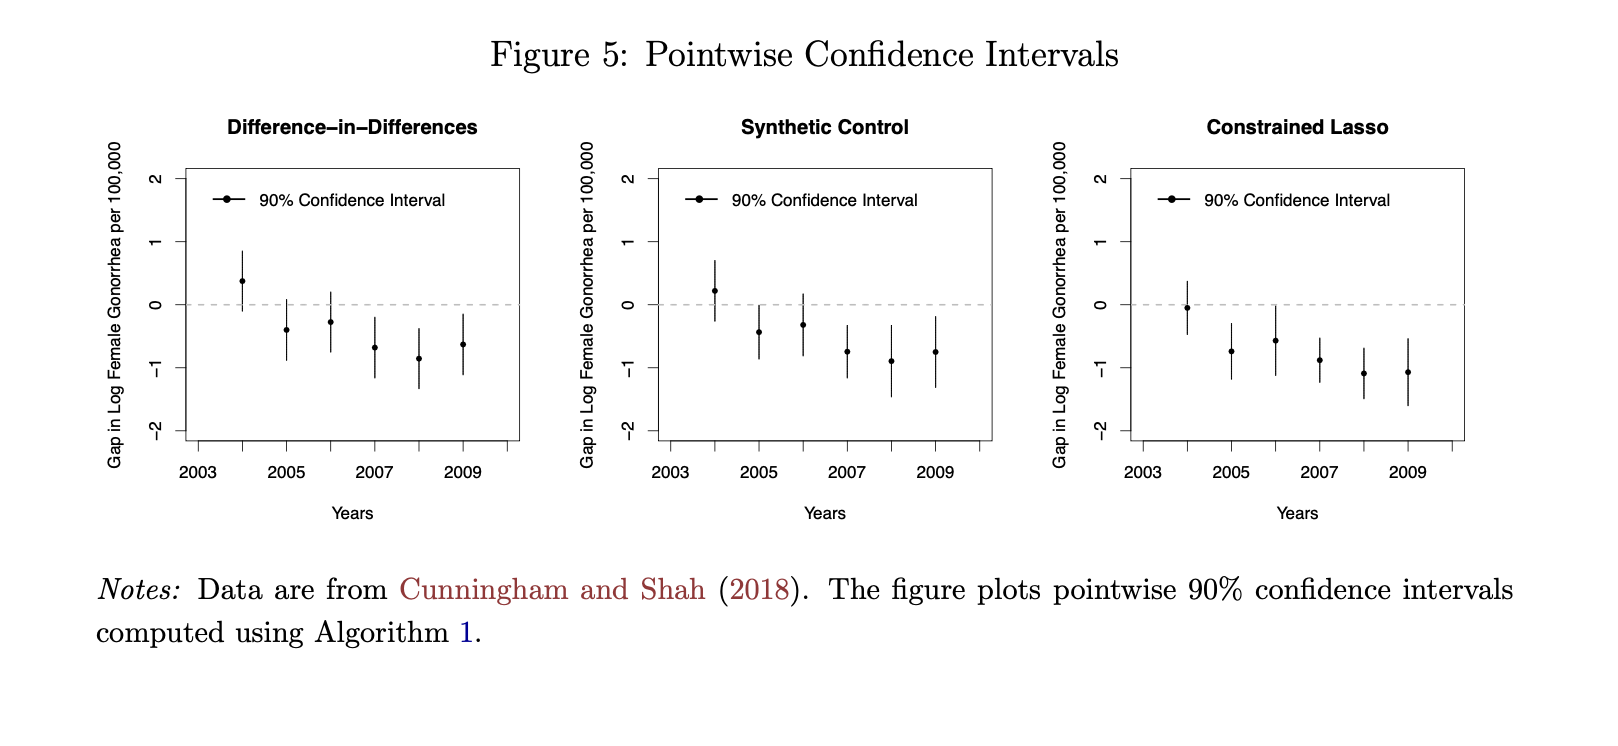
\includegraphics[width=0.7\linewidth]{./lecture_includes/figure5_conformal.png}
\end{center}

\end{frame}

\begin{frame}{Simulations}

\begin{itemize}
\item Now let's look at an example
\item Authors compare synth against ridge, Augmented synth with ridge regularization, demeaned synth, and fixed effects under four DGP
\item Augmenting synth with a ridge outcome regression reduces bias relative to synth alone in all four simulations
\item They also examine a real situation involving Kansas tax cuts in 2012
\end{itemize}

\end{frame}

\imageframe{./lecture_includes/aug_5.png}

\imageframe{./lecture_includes/aug_6.png}

\begin{frame}{Replication}

\begin{itemize}
\item We will now show code that does it in R and Stata
	\begin{itemize}
	\item R: "augsynth" by the authors
	\item Stata: "allsynth" that does several (including augsynth)
	\end{itemize}
\item Two examples to hopefully illustrate the bias and improvements and the lack of bias and no change in another \texttt{texas_augsynth.R} and \texttt{texas_allsynth.do}
	\begin{itemize}
	\item Smoking: augmented synth improves it
	\item Prisons: augmented synth does nothing
	\end{itemize}
\end{itemize}

\end{frame}



\begin{frame}{Augmented synth vs original synthetic control}

\begin{itemize}
\item In conclusion, synthetic control is best when pre-treatment fit is excellent, otherwise it is biased
\item Synthetic control avoids extrapolation by restricting weights to be non-negative and sum to one
\item Ridge regression augmentation will allow for a degree of extrapolation to achieve pre-treatment balance and that creates negative weights
\item Augmented synth will dominate synth in those instances by extrapolating outside the convex hull
\end{itemize}

\end{frame}






\subsection{Applying Machine Learning to Event studies from Finance}

\begin{frame}{Possibilities for detecting corruption}

\begin{itemize}

\item Event studies in finance have been used to detect abnormal patterns around ``events'' involving single firms
\item Baker and Gelbach (2020) proposes a type of synthetic control estimator that uses machine learning to estimate a counterfactual, as opposed to imposing strong parametric assumptions
\item Examples of its use have been applied to disruptions with the Elon Musk Twitter deal which while not corruption does involve estimating potential damages from stock price movements

\end{itemize}

\end{frame}

\begin{frame}{Largest Securities Class Action Settlements}

\begin{enumerate}

\item Enron: \$7.2b
\item WorldCom Inc: \$6.1b
\item Tyco International Ltd.: \$3.2b
\item Cendant Corporation: \$3.2b

\end{enumerate}

\end{frame}

\begin{frame}{Over time}

\begin{figure}
\includegraphics[scale=0.35]{./lecture_includes/baker_gelbach_1}
\end{figure}
\end{frame}

\begin{frame}{Event studies and securities litigation}

\begin{itemize}

\item Historically, the ``event study'' estimated ``abnormal'' returns under strong parametric assumptions (e.g., normality), but non-normal returns are normal

\begin{quote}
``The abnormal returns are the parameters that determine the damage estimates in securities suits, it is worthwhile to explore whether methods exist that can provide more accurate estimates of the abnormal return itself.''
\end{quote}

\item They argue that the event study is an out-of-sample prediction problem, which ML is used for, but it is also an extension of the synth modeling framework

\end{itemize}

\end{frame}

\begin{frame}{Basic idea}

\begin{figure}
\includegraphics[scale=0.35]{./lecture_includes/baker_gelbach_2}
\end{figure}
\end{frame}


\begin{frame}{Event studies as a prediction problem}

\begin{itemize}
\item Let the daily return for firm $i$ on date $t$ be $r_{i,t}$ and variables used for prediction is $X_{i,t}$ (e.g., market return, Fama-French and Carhart factors, a 1 for intercept, etc.)
\item Suppose an event reveals fraud.  It's effect on daily return is $r^1_{i,t} - r^0_{i,t}$ and we want to estimate $r^0_{i,t}$ with $\widehat{r}^0_{i,t}$
\item Construct a predicted residual as $\widehat{\varepsilon}_{i,t} = r_{i,t} - \widehat{r}^0_{i,t}$
\item Typically people would estimate this with OLS $$r_{i,t} = \alpha + \beta_1 X_{i,t} + \varepsilon_{i,t}$$
\end{itemize}

\end{frame}

\begin{frame}{OLS, ML, MSE, Bias, Variance}

\begin{itemize}
\item MSE of predicted abnormal return for $\widehat{\varepsilon}_{i,t} = r_{i,t} - \widehat{\beta}X_{i,t}$ is the sum of a squared bias term and a variance term
\item It's possible that the variance of one specification is lower enough than another to make up for a difference in bias
\item OLS also suffers because it overfits data when used for prediction -- it is best unbiased linear predictor but at the price of greater out-of-sample variance linear prediction
\item Since MSE is the basis for measuring prediction accuracy, ML estimators may outperform conventional OLS as we can explore increasing bias and reducing variance
\item ML methods accept bias in exchange for reduced variance out-of-sample accomplished through ``training''
\end{itemize}

\end{frame}

\begin{frame}{Paper's punchline}

\begin{quote}
``Using real stock return data, we demonstrate that a number of out-of-the-box statistical approaches that are relatively easy to interpret perform better than the standard, OLS-based event study specifications used in court proceedings.

\bigskip

We find that specifications using penalized regression generally perform well.  Specifications that adjust for daily market performance using data-driven peer indexes also generally perform well.

\bigskip

Finally, we obtain generally good performance from specifications that use a cross-validation technique that is robust to otherwise unmodeled time-series properties of the DGP. The best specifications provide noticeable improvements over event study approaches conventionally used in securities litigation. 

\end{quote}

\end{frame}

\begin{frame}{Peer index}

\begin{itemize}
\item They note that the best-performing specification makes use of both penalized regression and data-driven peer firm choice.
\item They call this the ``reasonable peer index'', and they show that ML methods can usefully serve as a basis for choosing \emph{which} peer firms to include in an event study (again, making this a synth-like method) which can mitigate the subjective researcher bias that synth is meant to overcome
\item Rather than subjectively picking which firms represent the counterfactual (over which there can be debate clearly, some disingenuous given the amount of money at stake), they propose letting the data say who the best peer is
\item But using \emph{any} peer index appears to mitigate this too
\end{itemize}

\end{frame}

\begin{frame}{Ranking all the ML methods}

\begin{figure}
\includegraphics[scale=0.35]{./lecture_includes/baker_gelbach_5}
\end{figure}
\end{frame}

\begin{frame}{Elon Musk example}

\begin{itemize}
\item In an unpublished analysis, Baker examined Elon Musk's attempt to buy Twitter on Twitter's stock price
\item Unlike his published paper, he's only going to use one form of ``penalized'' machine learning called ridge regression (which constrains what the coefficients can be in his model)
\item He will use peer index and the S\&P500 for prediction purposes
\end{itemize}

\end{frame}

\begin{frame}{Purpose of the exercise}

\begin{quote}
``The goal here is to get a rough estimate of what TWTR would be trading at had Elon never put the stock in play. Note, this does not mean that the prediction is equivalent to what TWTR would trade at were the deal to not go through (without any damage payments), as Elon has likely destroyed value in the process. This prediction could in fact be used as a baseline price in any tort-type damages claim that the company would want to bring against Elon after the process is over.''
\end{quote}

\end{frame}

\begin{frame}{Basic idea}

\begin{figure}
\includegraphics[scale=0.35]{./lecture_includes/baker_gelbach_3}
\end{figure}
\end{frame}

\begin{frame}{Basic idea}

\begin{figure}
\includegraphics[scale=0.35]{./lecture_includes/baker_gelbach_4}
\end{figure}
\end{frame}

\subsection{Concluding remarks}


\begin{frame}{Abadie on the value and use of synthetic control}

	\begin{figure}
	\includegraphics[scale=0.5]{./lecture_includes/abadie_quote.png}
	\end{figure}

\end{frame}



\section{Multiple Outcomes}

%--- Slide 1 ---
\begin{frame}{Motivation: A Tale of Two Californias}
  \begin{itemize}
    \item Recall from earlier the example wherein California in 1988 implemented strong anti-smoking laws—taxes, advertising bans, public campaigns.
    \item In Abadie et al. (2010), a "Synthetic California" was built to estimate the law's effect on smoking.
    \item Suppose we then asked: What about alcohol consumption?
    \begin{itemize}
      \item We'd construct a new synthetic California matched on pre-treatment alcohol trends.
      \item But we'd likely get different weights—different donor states.
    \end{itemize}
  \end{itemize}
\end{frame}

%--- Slide 2 ---
\begin{frame}{Interpretability Challenge}
  \begin{itemize}
    \item Now we have \textit{two} synthetic Californias:
    \begin{itemize}
      \item One built to predict smoking trends
      \item Another to predict alcohol trends
    \end{itemize}
    \item This breaks the narrative: which one is "the" counterfactual California?
    \item SCM aims to construct a unit-level counterfactual—not a new one for every outcome.
  \end{itemize}
\end{frame}

%--- Slide 3 ---
\begin{frame}{Why This Problem Matters More in SCM}
  \begin{itemize}
    \item Matching on covariates (e.g., Abadie \& Imbens) allows unit-specific matches—it's fine if donor sets vary.
    \item SCM differs: it promises to build one synthetic unit.
     \item If outcomes are driven by the same unobserved factors, we gain both interpretability and statistical efficiency by using common weights.
  \end{itemize}
\end{frame}


%--- Slide 1 ---
\begin{frame}{Motivation: SCM with Multiple Outcomes}
  \begin{itemize}
    \item Many SCM applications involve multiple outcomes, like arrests, violence and STIs (Cunningham and Shah 2018), employment and wages (Jardim, et al. 2022), etc.
    \item Standard practice is to estimate separate SCM weights for each outcome.
    \item Problem is that separate weights can (will?) yield very different donor pools \& make interpretation difficult.
  \end{itemize}
\end{frame}

%--- Slide 2 ---
\begin{frame}{Value-Add of This Paper}
  \begin{itemize}
    \item Sun, Ben-Michael, and Feller (2025) proposes methods to estimate a \textbf{common set of SCM weights} across outcomes.
    \item They'll present two approaches:
    \begin{itemize}
      \item Concatenated outcomes
      \item Averaged outcomes
    \end{itemize}
    \item Their goal is to lower bias \& get more interpretable synthetic units.
  \end{itemize}
\end{frame}

\begin{frame}{A Tension: Fit vs. Interpretability}
  \begin{block}{Audience Thought}
    \centering
    \large
    "If I separately optimized each outcome, won't any common set of weights necessarily fit \textbf{worse}?"
  \end{block}
  \vspace{0.5cm}
  \begin{itemize}
    \item Forcing a common set of weights improves interpretability—but may worsen pre-treatment fit.
    \item Separate SCM fits each outcome individually better—but sacrifices coherence.
    \item The real challenge: can we pool structure \textit{without} making both sides worse?
  \end{itemize}
\end{frame}


\begin{frame}{Separate SCM: Optimal for Each Outcome Individually}
  \begin{itemize}
    \item In separate SCM for outcome $k$, we solve:
    \[
    \min_{\gamma} \sum_{t=1}^{T_0} \left( Y_{1tk} - \sum_{i=2}^N \gamma_i Y_{itk} \right)^2
    \]
    subject to:
    \begin{itemize}
      \item $\sum_{i=2}^N \gamma_i = 1$ (weights sum to one)
      \item $\gamma_i \geq 0$ for all $i$ (non-negative weights)
    \end{itemize}
    \item Thus, the resulting weights are \textbf{optimal for outcome $k$} given these constraints.
    \item Without the non-negativity constraint, weights might sometimes be negative (as in some extensions like augmented SCM).
  \end{itemize}
\end{frame}




\begin{frame}{Reminder: Pre-Treatment Fit}
  \begin{itemize}
    \item In SCM, even the best possible weights usually leave some \textbf{residual discrepancy}.
    \item $q(\gamma)$ measures the pre-treatment gap between the treated unit and the synthetic control.
    \item Smaller $q(\gamma)$ $\Rightarrow$ better fit, but perfect match is rare given real-world donor pools.
  \end{itemize}
  \vspace{0.5cm}
  \begin{center}
  \includegraphics[width=0.65\linewidth]{./lecture_includes/reminder_fit.png}
  \end{center}
\end{frame}

\begin{frame}{A New Optimization Problem: Global Coherence}
  \begin{itemize}
    \item Sun, Ben-Michael, and Feller (2025) propose not just a new estimator, but a \textbf{new objective}.
    \item Minimize pre-treatment discrepancy \textbf{across outcomes simultaneously} by optimizing a \textit{pooled} loss:
  \end{itemize}
  \[
    \min_{\gamma} \left\{ \nu \cdot q_{\text{avg}}(\gamma) + (1 - \nu) \cdot q_{\text{cat}}(\gamma) \right\}
  \]
  \begin{itemize}
    \item Where:
    \begin{itemize}
      \item $q_{\text{avg}}(\gamma)$ minimizes discrepancy for the average of outcomes.
      \item $q_{\text{cat}}(\gamma)$ minimizes discrepancy across all outcomes stacked together.
    \end{itemize}
    \item The resulting common weights are \textbf{optimal for this new pooled objective}—not for any single outcome’s individual fit.
  \end{itemize}
\end{frame}

%--- Slide 3 ---
\begin{frame}{Setup and Target Parameter}
  \begin{itemize}
  \item Recall that Abadie used $J$ for the number of donor units by here Sun, Ben-Michael, and Feller (2025) use $N$ for total units and $N_0$ for donor units.

    \item One treated unit, $N-1$ control units, $K$ outcomes.
    \item Interested in post-treatment effects $\tau_k = Y_{1T,k}(1) - Y_{1T,k}(0)$.
    \item SCM estimates $Y_{1T,k}(0)$ using weighted average of donor pool units.
  \end{itemize}
\end{frame}

\begin{frame}{Demeaned estimator}

\begin{quote}
“We follow the potential outcomes framework … and throughout focus on de-meaned or intercept-shifted weighting estimators, which were introduced in the single outcome setting (Doudchenko and Imbens, 2017; Ferman and Pinto, 2021) and were adapted to multiple outcomes by Tian et al. (2023), who argue that outcome-specific demeaning is useful for comparing across outcomes.” -- Sun, Ben-Michael and Feller (2025)
\end{quote}

\end{frame}

%--- Slide 4 ---
\begin{frame}{Estimator Form}
  \begin{itemize}
    \item Demeaned estimator:
    \[
    \hat{Y}_{1T,k}(0) = \bar{Y}_{1\cdot k} + \sum_{i=2}^N \gamma_i (Y_{iT,k} - \bar{Y}_{i\cdot k})
    \]
    \item Where:
    \begin{itemize}
      \item $\bar{Y}_{1\cdot k}$ is the treated unit’s pre-treatment average for outcome $k$.
      \item $\bar{Y}_{i\cdot k}$ is control unit $i$'s pre-treatment average for outcome $k$.
      \item $(Y_{iT,k} - \bar{Y}_{i\cdot k})$ is the deviation of control unit $i$'s post-treatment outcome from its pre-treatment mean.
      \item $\gamma_i$ are the donor pool weights chosen to best match pre-treatment trajectories.
    \end{itemize}
    \item We choose weights $\gamma$ to minimize pre-treatment imbalance.
    \item \textbf{Key difference:} How we define imbalance when $K > 1$.
  \end{itemize}
\end{frame}

%--- Slide 5 ---
\begin{frame}{Problems with Separate Weights}
  \begin{itemize}
    \item Each outcome gets its own set of SCM weights.
    \item Can lead to overfitting, especially in short panels.
    \item Different donors per outcome $\Rightarrow$ hard to interpret one synthetic unit.
  \end{itemize}
  \includegraphics[width=0.9\linewidth]{./lecture_includes/figure1_weights.png}
\end{frame}

%--- Slide 6 ---
\begin{frame}{Proposed Solution: Shared Weights}
  \begin{itemize}
    \item Estimate a \textbf{common set of weights} across outcomes.
    \item Two strategies:
    \begin{itemize}
      \item \textbf{Concatenated:} stack all outcome-time pairs.
      \item \textbf{Averaged:} average outcomes before computing imbalance.
    \end{itemize}
  \end{itemize}
\end{frame}

%--- Slide 7 ---
\begin{frame}{Formalizing the Objective Functions}
  \begin{itemize}
    \item Concatenated weights minimize:
    \[ q_{\text{cat}}(\gamma)^2 = \frac{1}{T_0 K} \sum_{k=1}^K \sum_{t=1}^{T_0} \left(Y_{1tk} - \sum_{i=2}^N \gamma_i Y_{itk} \right)^2 \]
    \item Averaged weights minimize:
    \[ q_{\text{avg}}(\gamma)^2 = \frac{1}{T_0} \sum_{t=1}^{T_0} \left( \frac{1}{K} \sum_{k=1}^K Y_{1tk} - \sum_{i=2}^N \gamma_i \frac{1}{K} \sum_{k=1}^K Y_{itk} \right)^2 \]
  \end{itemize}
\end{frame}

%--- Slide 8 ---
\begin{frame}{Why Averaging Helps}
  \begin{itemize}
    \item Averaging outcomes smooths out idiosyncratic noise.
    \item Leads to tighter fit and lower bias bounds as $K$ grows.
    \item Bias bound: $O(1/\sqrt{K})$ under low-rank factor model.
  \end{itemize}
\end{frame}

%--- Slide 9 ---
\begin{frame}{Key Assumption: Low-Rank Structure}
  \begin{itemize}
    \item Outcomes are driven by common latent factors:
    \[ L_{itk} = \phi_i^\top \mu_{tk} \]
    \item Oracle weights exist iff the data matrix is low rank.
    \item Factor model aligns donor units via shared structure.
  \end{itemize}
\end{frame}

%--- Slide 10 ---
\begin{frame}{Bias Decomposition}
  \begin{itemize}
    \item Total estimation error = bias + noise
    \item Bias: failure to balance latent structure
    \item Noise: post-treatment idiosyncratic error
  \end{itemize}
\end{frame}

%--- Slide 11 ---
\begin{frame}{Theorem 1: Bias Bounds}
  \begin{itemize}
    \item Separate SCM: $O(1)$ bias
    \item Concatenated SCM: $O(1)$, better overfitting control
    \item Averaged SCM: $O(1/\sqrt{K})$ bias
  \end{itemize}
  \includegraphics[width=0.9\linewidth]{./lecture_includes/table1_bounds.png}
\end{frame}

%--- Slide 12 ---
\begin{frame}{Practical Diagnostics}
  \begin{itemize}
    \item Singular value decomposition (SVD): do a few components explain most variation?
    \item Hold-out fit: leave one outcome out and check fit.
    \item Combine averaging and concatenation (weighted frontier).
  \end{itemize}
\end{frame}

%--- Slide 13 ---
\begin{frame}{Application: Flint Water Crisis}
  \begin{itemize}
    \item Flint is treated unit; 54 MI school districts as controls.
    \item 4 outcomes: math, reading, attendance, special needs.
    \item Estimate SCM using separate, cat., avg., and combined weights.
  \end{itemize}
  \includegraphics[width=0.9\linewidth]{./lecture_includes/figure2_gaps.png}
\end{frame}

%--- Slide 14 ---
\begin{frame}{Flint Results: Interpretation}
  \begin{itemize}
    \item Separate weights fit very well pre-treatment but likely overfit.
    \item Average and combined weights offer good fit with less overfitting.
    \item Estimated impacts: decline in math scores, increase in special needs.
  \end{itemize}
\end{frame}

%--- Slide 15 ---
\begin{frame}{Simulation: Clean vs. Noisy Outcomes}
  \begin{itemize}
    \item Vary strength of shared vs. idiosyncratic factors.
    \item When outcomes share structure: avg. \& cat. reduce bias.
    \item When outcomes diverge: separate may be safer.
  \end{itemize}
  \includegraphics[width=0.9\linewidth]{./lecture_includes/sim1_bias_boxplots.png}
\end{frame}

%--- Slide 16 ---
\begin{frame}{Simulation: Failure Case}
  \begin{itemize}
    \item When $\rho = 0$, no shared structure $\Rightarrow$ avg. SCM fails.
    \item Bias explodes as averaging collapses signal.
    \item Use SVD or condition number to detect weak structure.
  \end{itemize}
  \includegraphics[width=0.9\linewidth]{./lecture_includes/sim2_failure_case.png}
\end{frame}

%--- Slide 17 ---
\begin{frame}{Recommendations for Practice}
  \begin{itemize}
    \item Standardize outcomes.
    \item Check SVD or hold-out diagnostics.
    \item Use average or combined weights when K is large and shared structure is plausible.
  \end{itemize}
\end{frame}

%--- Slide 18 ---
\begin{frame}{Combined Objective Frontier}
  \begin{itemize}
    \item Blend average and concatenated objectives.
    \item Tune $\nu$ to balance fit and robustness.
    \item Visual: \texttt{augsynth} package frontier plot
  \end{itemize}
  \includegraphics[width=0.85\linewidth]{./lecture_includes/frontier_plot.png}
\end{frame}

%--- Slide 19 ---
\begin{frame}{Why This Paper Matters}
  \begin{itemize}
    \item Pushes SCM beyond single-outcome constraint.
    \item Improves interpretability and bias control.
    \item Leads naturally into matrix completion \& machine learning SCM.
  \end{itemize}
\end{frame}

%--- Slide 20 ---
\begin{frame}{Questions?}
  \begin{itemize}
    \item Let’s discuss diagnostics, estimation details, or extensions.
    \item Also happy to talk about \texttt{augsynth} implementation.
  \end{itemize}
\end{frame}



\section{Multiple Treated Units and Staggered}





\subsection{Matrix completion with nuclear norm}

\begin{frame}{Big idea}

\begin{quote}
``To estimate average causal effect of the treatment on the treated units, we impute the missing potential control outcomes'' -- Athey, et al. (2021)
\end{quote}

\bigskip

All of causal inference is imputation -- but some methods are more explicit and do so in a way that layers on stronger assumptions than others -- and matrix completion with nuclear norm regularization is one such example. 


\end{frame}

\begin{frame}{Matrix Completion with Nuclear Norm Regularization}
\small
\begin{itemize}
  \item Athey et al. (2021) propose matrix completion as a generalization of SCM and DiD.
  \item Uses nuclear norm regularization to encourage low-rank structure without specifying the number of factors.
  \item Flexible enough to handle staggered adoption and complex missingness patterns.
  \item Outperforms standard SCM and DiD in simulations.
\end{itemize}

\end{frame}

\begin{frame}{What is Matrix Completion?}
\small
\begin{itemize}
  \item Matrix completion means filling in missing entries of a matrix.
  \item In causal inference, the "missing entries" are missing potential outcomes (e.g., $Y^0$ for treated units).
  \item When we estimate the ATT, we are trying to impute missing counterfactual outcomes.
\end{itemize}
\end{frame}



\begin{frame}{The Netflix Prize and Matrix Completion}
\small
\begin{itemize}
  \item In 2006, Netflix offered \$1 million to improve its movie recommendation algorithm.
  \item Problem: A giant, sparse matrix of users and movie ratings.
  \item Task: Predict missing entries — "If you haven't rated \underline{Napoleon Dynamite}, would you like it?"
  \item Matrix completion techniques — low-rank approximations — became key to solving this.
\end{itemize}
\end{frame}



\begin{frame}{Why Netflix's Problem Was Implicitly Causal}
\small
\begin{itemize}
  \item Netflix wasn't just predicting preferences — it was asking:
  \[
  \text{If we show you \underline{Napoleon Dynamite}, will you like it?}
  \]
  \item Matrix completion predicted missing outcomes under interventions.
  \item In causal inference, we face the same problem:  
  \[
  \text{What would have happened to treated units had they not been treated?}
  \]
\end{itemize}
\end{frame}



\begin{frame}{Roadmap: From Missing Outcomes to Matrix Completion}

\begin{itemize}
  \item Causal inference often reduces to \textbf{imputing missing potential outcomes}.
  \item Different designs (DiD, SCM) create different \textbf{missingness patterns}.
  \item Whether the matrix is "thin" or "fat" shapes the \textbf{regression strategy} for imputation.
  \item \textbf{Matrix Completion with Nuclear Norm Regularization} generalizes across both traditions.
\end{itemize}

\begin{center}
\includegraphics[width=0.5\linewidth]{./lecture_includes/flowchart.png}
\end{center}
\end{frame}



\begin{frame}[plain]
\small
Here's a matrix of untreated potential outcomes, $Y^0$, representing units over time periods $t$:
\begin{center}
\[
Y^0_{it} = \begin{pmatrix}
Y^0_{11} & Y^0_{12} & Y^0_{13} & \dots & Y^0_{1t} \\
Y^0_{21} & Y^0_{22} & Y^0_{23} & \dots & Y^0_{2t} \\
\vdots & \vdots & \vdots & \ddots & \vdots \\
Y^0_{i1} & Y^0_{i2} & Y^0_{i3} & \dots & Y^0_{it}
\end{pmatrix}
\]
\end{center}

Now imagine a treatment assigned in the last period $t$, according to the switching equation:
\[
Y = DY^1 + (1-D)Y^0
\]
\end{frame}



\begin{frame}[plain]
\small
Since treatment occurs in the last period, we are missing the untreated potential outcomes for the treated units:

\begin{center}
\[
Y^0_{it} = \begin{pmatrix}
Y^0_{11} & Y^0_{12} & Y^0_{13} & \dots & ? \\
Y^0_{21} & Y^0_{22} & Y^0_{23} & \dots & ? \\
\vdots & \vdots & \vdots & \ddots & \vdots \\
Y^0_{i1} & Y^0_{i2} & Y^0_{i3} & \dots & ?
\end{pmatrix}
\]
\end{center}

\end{frame}




\begin{frame}[plain]
\small
Matrix completion with nuclear norm regularization imputes the missing entries:

\begin{center}
\[
Y^0_{it} = \begin{pmatrix}
Y^0_{11} & Y^0_{12} & Y^0_{13} & \dots & \widehat{Y^0_{1t}} \\
Y^0_{21} & Y^0_{22} & Y^0_{23} & \dots & \widehat{Y^0_{2t}} \\
\vdots & \vdots & \vdots & \ddots & \vdots \\
Y^0_{i1} & Y^0_{i2} & Y^0_{i3} & \dots & \widehat{Y^0_{it}}
\end{pmatrix}
\]
\end{center}

Once we have the imputed untreated outcomes, we can calculate individual treatment effects and aggregate to the ATT.
\end{frame}





\begin{frame}{Two Traditions in Causal Inference}
\small
 In causal inference, we often come from two traditions: unconfoundedness or synthetic control

\begin{itemize}
  \item \textbf{Unconfoundedness}: $(Y^0, Y^1) \perp D | X$ (propensity score, matching, DiD).
  \item \textbf{Synthetic Control}: Match pre-treatment outcomes directly by reweighting donor units.
  \item Matrix completion with nuclear norm (MC-NNM) nests both within a broader low-rank modeling framework.
\end{itemize}
\end{frame}




\begin{frame}{Different Stability Assumptions}
\small
\begin{itemize}
  \item \textbf{Unconfoundedness}: Assumes patterns over time are stable across units.
  \item \textbf{Synthetic Control}: Assumes patterns across units are stable over time.
  \item MC-NNM uses regularization (nuclear norm) to interpolate missing outcomes under either kind of stability.
\end{itemize}
\end{frame}



\begin{frame}{Contributions of Matrix Completion (MC-NNM)}
\small
\begin{enumerate}
  \item Provides formal results under non-random missingness with block structure (e.g., staggered adoption).
  \item Shows that unconfoundedness and synthetic control are special cases of matrix completion.
  \item Proposes nuclear norm regularization to recover low-rank structure without rigid restrictions.
\end{enumerate}
\end{frame}


\begin{frame}{What Is a Low-Rank Matrix?}
\small
\begin{itemize}
  \item A matrix is \textbf{low-rank} if it can be well-approximated by a small number of underlying patterns (factors).
  \item Example:
    \begin{itemize}
      \item Suppose states' education outcomes are driven by just two things:
      \begin{itemize}
        \item (1) Overall economic prosperity,
        \item (2) Strength of state education policy.
      \end{itemize}
      \item Then a big matrix of outcomes across states and years has \textbf{only two hidden factors}.
    \end{itemize}
\end{itemize}
\end{frame}


\begin{frame}{Low-Rank vs. High-Rank Matrices}
\small
\begin{itemize}
  \item \textbf{Low-Rank Matrix}:
  \begin{itemize}
    \item Outcomes across units and time are driven by a few common forces.
    \item Missing outcomes can be reliably imputed by recovering those forces.
    \item \textit{(Example: Economic prosperity + state policy explain education scores.)}
  \end{itemize}
  \vspace{0.3cm}
  \item \textbf{High-Rank Matrix}:
  \begin{itemize}
    \item Every unit-time pair varies independently.
    \item No simple pattern or structure across the matrix.
    \item Imputation becomes almost impossible — you're just guessing noise.
    \item \textit{(Example: Every state's education outcomes fluctuate wildly for unique, idiosyncratic reasons.)}
  \end{itemize}
\end{itemize}
\end{frame}



\begin{frame}{Missingness Patterns in Causal Inference}
\small
\begin{itemize}
  \item In causal inference, we often work with matrices of outcomes — some entries are missing because of treatment.
  \item Different designs create different patterns of missingness:
  \begin{itemize}
    \item \textbf{Unconfoundedness}: missing outcomes only after treatment.
    \item \textbf{Staggered adoption or event studies}: missingness varies across units and periods.
    \item \textbf{Synthetic control}: typically missing a treated unit’s potential outcomes after a specific intervention.
  \end{itemize}
\end{itemize}
\end{frame}




\begin{frame}{Single Treated-Period Block Structure (Unconfoundedness)}
\small
\begin{itemize}
  \item Under unconfoundedness, missing outcomes occur only in the post-treatment period.
  \item Example: LaLonde (1986) — National Supported Work program (NSW).
  \begin{itemize}
    \item Treated workers are missing untreated earnings outcomes in the final period.
    \item Use comparison group outcomes to impute missing potential outcomes.
  \end{itemize}
  \item Athey et al. call this the ``single treated-period block structure''.
\end{itemize}
\end{frame}



\begin{frame}{Single-treated-period block structure}

\begin{center}
\[ Y^0_{it}  =\begin{pmatrix}
    Y^0_{11} & Y^0_{12} & Y^0_{13} & \dots  &Y^0_{1T} \\
    Y^0_{21} & Y^0_{22} & Y^0_{23} & \dots  & ? \\
    \vdots & \vdots & \vdots & \ddots & \vdots \\
    Y^0_{i1} & Y^0_{i2} & Y^0_{i3} & \dots  & ?
\end{pmatrix}\]
\end{center}

\end{frame}


\begin{frame}{Single-\textcolor{green}{treated-unit} block structure}

\begin{center}
\[ Y^0_{it}  =\begin{pmatrix}
    Y^0_{11} & Y^0_{12} & Y^0_{13} & \dots  & Y^0_{1t} \\
    Y^0_{21} & Y^0_{22} & Y^0_{23} & \dots  & Y^0_{2t}  \\
    \vdots & \vdots & \vdots & \ddots & \vdots \\
    Y^0_{i1} & Y^0_{i2} & ? & \dots  & ?
\end{pmatrix}\]
\end{center}

Notice, this is the synthetic control design because a single unit (unit $i$) is missing $Y^0$ for the 3rd and $t$th periods.

\end{frame}

\begin{frame}{Differential timing has a block structure too}

\begin{center}
\[ Y^0_{it}  =\begin{pmatrix}
    Y^0_{11} & ? & ? & \dots  & ? \\
    Y^0_{21} & Y^0_{22} & Y^0_{23} & \dots  & ? \\
    \vdots & \vdots & \vdots & \ddots & \vdots \\
    Y^0_{i1} & Y^0_{i2} & ? & \dots  & ?
\end{pmatrix}\]
\end{center}

So all of these so-called designs can be expressed in terms of missingness in the block structure, and our job therefore is to find an estimator that is general enough to manage all of them.  Matrix completion with nuclear norm regularization is one such example and so has nice generalizations

\end{frame}


\begin{frame}{Why Matrix Shape Matters for Imputation}

\begin{itemize}
\item Next we must consider the relative number of panel units $N$ and time periods $T$ because this also shapes which regression style will be used for imputation
\item Thin matrices are where $N>>T$ (relatively large numbers of units), and fat matrices are ones where $T>>N$ (relatively large numbers of time periods)
\item Approximately square ones are where $T$ is approximately equal to $N$
\end{itemize}

\end{frame}


\begin{frame}{Horizontal Regression}
\small
\begin{itemize}
  \item Under unconfoundedness, we have a "thin" matrix: many units ($N$) but few periods ($T$).
  \item Horizontal regression means regressing across units:
  \[
  Y_{iT} \sim X_i
  \]
  where $X_i$ are pre-treatment outcomes or covariates for unit $i$.
  \item Horizontal regression uses large $N$ to impute missing $Y^0$ at $T$.
\end{itemize}
\end{frame}




\begin{frame}{Vertical Regression}
\small
\begin{itemize}
  \item In synthetic control, we match across time for a single treated unit.
  \item Vertical regression regresses the treated unit’s pre-treatment outcomes onto donor units’ pre-treatment outcomes:
  \[
  Y_{1t} \sim Y_{2t}, Y_{3t}, \dotsc, Y_{Nt} \quad \text{(for } t=1,\dotsc,T_0 \text{)}
  \]
  \item Synthetic control imposes:
  \begin{itemize}
    \item Non-negative weights,
    \item Weights sum to one.
  \end{itemize}
\end{itemize}
\end{frame}




\begin{frame}{Fixed effects and factor models}

\begin{itemize}
\item Both horizontal and vertical regressions exploit unique patterns in the data -- one goes left to right, one goes up and down
\item An alternative is to combine both stable patterns across units and across time.
\item Matrix completion with nuclear norm regularization (MC-NNM) does this by leveraging low-rank structure.
\end{itemize}

\end{frame}


\begin{frame}{Matrix Completion Model}
\small
\begin{itemize}
\item Model the $N \times T$ matrix of outcomes as:
\[
Y = L^* + e
\]
\item $E[e|L^*]=0$, $e$ can be thought of as idiosyncratic noise or measurement error and $L^*$ is the "true" low-rank structure we want to recover.
\end{itemize}
\end{frame}



\begin{frame}{Error Assumptions}
\small
\begin{block}{Matrix Assumptions}
$e$ is independent of $L^*$, and the elements of $e$ are $\sigma$-sub-Gaussian and independent across cells.
\end{block}

Sub-Gaussian means the error has light tails (bounded variability), like a normal distribution, which controls large deviations.

\end{frame}



\begin{frame}{Why Regularization is Needed}
\small
\begin{itemize}
\item Without regularization, the estimator would just return $Y$ and ignore structure ($\delta = 0$).
\item We add a penalty on the complexity of $L^*$ to encourage low-rank recovery.
\item Different penalties exist — MC-NNM uses the nuclear norm, not lasso or elastic net.
\end{itemize}
\end{frame}


\begin{frame}{What Does "Norm" Mean?}
\small
\begin{itemize}
  \item A \textbf{norm} measures the size or magnitude of a vector or matrix.
  \item In synthetic control:
  \[
  \|X_1 - X_0 W\| \quad \text{measures pre-treatment fit (squared discrepancies)}
  \]
  \item In matrix completion:
  \[
  \|L\|_* \quad \text{(nuclear norm) measures complexity (sum of singular values)}
  \]
  \item Norms inside the objective function measure how big the error is;
  Norms inside the penalty term measure how complex the solution is.
\end{itemize}
\end{frame}

\begin{frame}{Illustrating the Frobenius and Nuclear Norms}
\small
\[
A = \begin{pmatrix}
a_{11} & a_{12} & a_{13} \\
a_{21} & a_{22} & a_{23}
\end{pmatrix}
\]

\bigskip

\begin{itemize}
  \item \textbf{Frobenius norm} $\|A\|_F$:
  \[
  \|A\|_F = \sqrt{a_{11}^2 + a_{12}^2 + a_{13}^2 + a_{21}^2 + a_{22}^2 + a_{23}^2}
  \]
  Measures the overall size (energy) of the matrix.
  
  \item \textbf{Nuclear norm} $\|A\|_*$:
  \[
  \|A\|_* = \text{sum of singular values of } A
  \]
  Measures the complexity (effective number of dimensions) of the matrix.
\end{itemize}
\end{frame}

\begin{frame}{Key Idea Before the Estimator}
\small
\begin{itemize}
  \item Two things matter in matrix completion:
  \begin{itemize}
    \item \textbf{Fit}: How well we match the observed outcomes (measured by Frobenius norm).
    \item \textbf{Simplicity}: How simple the underlying structure is (measured by Nuclear norm).
  \end{itemize}
  \item The estimator balances these two goals:
  \begin{itemize}
    \item Match the observed data well,
    \item Keep the solution simple and low-rank.
  \end{itemize}
\end{itemize}
\end{frame}



\begin{frame}{Key Idea Before the Estimator}
\small
\begin{itemize}
  \item Two things matter in matrix completion:
  \begin{itemize}
    \item \textbf{Fit}: How well we match the observed outcomes (measured by Frobenius norm).
    \item \textbf{Simplicity}: How simple the underlying structure is (measured by Nuclear norm).
  \end{itemize}
  \item The estimator balances these two goals:
  \begin{itemize}
    \item Match the observed data well,
    \item Keep the solution simple and low-rank.
  \end{itemize}
\end{itemize}
\end{frame}



\begin{frame}{Estimator Formulation}
\small

$$L^* = \widehat{L} + \widehat{\Gamma} 1_T^T + 1_N \widehat{\Delta}^T$$
\bigskip

Objective:
$$ \arg\min_{L, \Gamma, \Delta} \left\{ \frac{1}{O} \|P_0(Y - L - \Gamma 1_T^T - 1_N \Delta^T)\|_F^2 + \Lambda \|L\|_* \right\}$$

where $\|\cdot\|_F$ is Frobenius norm, $\|\cdot\|_*$ is nuclear norm.
\end{frame}




\begin{frame}{Fixed Effects and Regularization}
\small
\begin{itemize}
\item Fixed effects ($\Gamma$, $\Delta$) are \textbf{not} penalized — only $L$ is regularized.
\item This separation helps when the fraction of observed outcomes is relatively large.
\item The nuclear norm penalty is chosen via cross-validation.
\item Advantage: convex optimization is fast and reliable even when $N$ or $T$ is large.
\end{itemize}
\end{frame}

\begin{frame}{Recap: What Matrix Completion Does}
\small
\begin{itemize}
  \item Matrix completion with nuclear norm (MC-NNM) estimates missing potential outcomes.
  \item It balances two goals:
  \begin{itemize}
    \item \textbf{Fit}: Match observed outcomes (Frobenius norm).
    \item \textbf{Simplicity}: Keep the structure low-rank (Nuclear norm).
  \end{itemize}
  \item It generalizes synthetic control and difference-in-differences.
  \item Now, we'll see how to actually estimate it in practice.
\end{itemize}
\end{frame}




\begin{frame}{fect code for MCNN}

fect in R: \url{https://github.com/xuyiqing/fect}

\bigskip

fect in Stata: \url{https://yiqingxu.org/packages/fect/stata/fect_md.html}

\end{frame}





\subsection{Synthetic difference-in-differences}

\begin{frame}{Motivation for Synthetic DiD}
\small
\begin{itemize}
  \item Difference-in-Differences (DiD) assumes parallel trends but can fail if treated units and controls are too different.
  \item Synthetic Control (SC) matches treated units better, but struggles with few pre-treatment periods or noisy data.
  \item \textbf{Synthetic Difference-in-Differences (SDID)} combines strengths of both:
  \begin{itemize}
    \item Matches pre-treatment trends (SC),
    \item Adjusts for common time trends (DiD).
  \end{itemize}
\end{itemize}
\end{frame}




\begin{frame}{Big Picture: What SDID Does}
\small
\begin{itemize}
  \item \textbf{Unit Weights}: Match treated units to control units (like Synthetic Control).
  \item \textbf{Time Weights}: Adjust for changing trends over time (like DiD).
  \item \textbf{Goal}: Achieve better balance across units and time without assuming perfect parallel trends.
\end{itemize}
\end{frame}




\begin{frame}{Key Assumptions Behind SDID}
\small
\begin{itemize}
  \item Large number of control units and pre-treatment periods.
  \item Systematic trends (latent factors) can be well-approximated by a low-rank structure.
  \item Errors are light-tailed and roughly independent across cells.
\end{itemize}
\end{frame}


\begin{frame}{Key Assumptions Behind SDID}
\small
\begin{itemize}
  \item \textbf{1. Light-Tailed Errors}: Random shocks are not too wild (no extreme outliers).
  \item \textbf{2. Sufficient Data}: Enough control units and pre-treatment periods to estimate trends reliably.
  \item \textbf{3. Low-Rank Structure}: Systematic trends can be explained by a few hidden patterns (not too complicated).
  \item \textbf{4. Good Balancing}: The unit and time weights can correct for trend differences without needing perfect matching.
\end{itemize}
\end{frame}


\begin{frame}{Unit and Time Weights: Intuition}
\small
\begin{itemize}
  \item \textbf{Unit Weights (\(\hat{w}\))}: 
  Build a weighted combination of control units to match treated units before treatment.
  \item \textbf{Time Weights (\(\hat{\lambda}\))}: 
  Prioritize pre-treatment periods that are most predictive for post-treatment behavior.
  \item \textbf{Goal}: 
  Create a flexible, balanced counterfactual that adjusts across units and time.
\end{itemize}
\end{frame}



\begin{frame}{Estimating Unit and Time Weights}
\small
\begin{itemize}
  \item \textbf{Unit Weights (\(\hat{w}\))}: 
  \begin{itemize}
    \item Estimated via constrained least squares to match pre-treatment outcomes.
    \item Non-negative, sum to one (plus regularization).
  \end{itemize}
  \item \textbf{Time Weights (\(\hat{\lambda}\))}: 
  \begin{itemize}
    \item Estimated via constrained least squares to prioritize informative pre-treatment periods.
  \end{itemize}
  \item \textbf{Regularization}: 
  \begin{itemize}
    \item Aligns regularization strength with typical one-period changes among untreated units:
    \[
    \Delta_{it} = Y_{i(t+1)} - Y_{it}
    \]
    \item Prevents overfitting and ensures generalization.
  \end{itemize}
\end{itemize}
\end{frame}

\begin{frame}{Steps in SDID Estimation}
\small
\begin{itemize}
  \item Step 1: Identify unit weights (\(\hat{w}\)) to match treated and control units pre-treatment.
  \item Step 2: Identify time weights (\(\hat{\lambda}\)) to balance trends across periods.
  \item Step 3: Combine unit and time weights in a weighted regression to estimate ATT.
\end{itemize}
\end{frame}








\begin{frame}{Outcome Model Behind SDID}
\small
\[
Y = L + D \circ \delta + E
\]
\begin{itemize}
  \item \(L\): Systematic trends across units and time (e.g., shared economic factors).
  \item \(D \circ \delta\): Treatment effects applied selectively to treated units and periods.
  \item \(E\): Idiosyncratic noise.
\end{itemize}
\end{frame}


\begin{frame}{Oracle vs. Empirical Weights}
\small
\begin{itemize}
  \item \textbf{Oracle Weights}: Theoretical best weights that perfectly balance \(L\) (systematic trends).
  \item \textbf{Empirical Weights}: Estimated from the data, approximate the oracle weights.
  \item Goal: Pre-treatment balance without needing perfect matches or perfect parallel trends.
\end{itemize}
\end{frame}





\begin{frame}{Combined SDID Estimation}
\small
\[
\text{argmin}_{\tau, \mu, \alpha, \beta} \sum_{i=1}^N \sum_{t=1}^T (Y_{it} - \mu - \alpha_i - \beta_t - W_{it} \tau)^2 \hat{w}_i \hat{\lambda}_t
\]
\begin{itemize}
  \item Combines unit and time weights in a weighted regression.
  \item Matches treated and control units, adjusting across units and time.
  \item Ensures counterfactual trends are well aligned without assuming perfect parallel trends.
\end{itemize}
\end{frame}



\begin{frame}{Regression Comparison: SC, DiD, SDiD}

\begin{itemize}
    \item Synthetic Control (SC):
    \[
    \tau^{\text{SC}} = \textrm{argmin}_{\tau, \lambda} \sum_{i,t} (Y_{it} - \lambda_t - \tau D_{it})^2 w_i^{\text{SC}}
    \]
    \item Difference-in-Differences (DiD):
    \[
    \text{argmin}_{\tau, \lambda, \alpha} \sum_{i,t} (Y_{it} - \lambda_t - \alpha_i - \tau D_{it})^2
    \]
    \item Synthetic Difference-in-Differences (SDiD):
    \[
    \text{argmin}_{\tau, \lambda, \alpha} \sum_{i,t} (Y_{it} - \lambda_t - \alpha_i - \tau D_{it})^2 w_i \lambda_t
    \]
\end{itemize}

\end{frame}

\begin{frame}{Key Features of SDiD}

\begin{itemize}
    \item Combines synthetic control's matching with DID's parallel trends adjustment.
    \item Introduces unit and time weights for improved balance.
    \item Does not require perfect pre-treatment matching or strictly parallel trends.
\end{itemize}

\end{frame}




\begin{frame}{Decomposing the Bias of SDiD}
\[
\widehat{\tau}^{sdid} - \tau = \varepsilon(\widetilde{w}, \widetilde{\lambda}) + B(\widetilde{w}, \widetilde{\lambda}) + \widehat{\tau}(\widehat{w},\widehat{\lambda}) - \widehat{\tau}(\widetilde{w},\widetilde{\lambda})
\]
\begin{itemize}
\item \textbf{Oracle noise}: Variance introduced by weights and sample limitations.
\item \textbf{Oracle confounding bias}: Systematic differences not removed by weights.
\item \textbf{Deviation from oracle}: Approximation errors in empirical weights.
\end{itemize}
\end{frame}

\begin{frame}{Oracle Noise}
\begin{itemize}
\item Noise arises from random variation in data.
\item Small when weights (\(\hat{w}, \hat{\lambda}\)) are small and sample sizes are sufficient.
\item Ensures noise does not dominate the estimator.
\end{itemize}
\end{frame}

\begin{frame}{Oracle Confounding Bias: Units and Time}
\begin{itemize}
\item \textbf{Units (Rows)}:
    \[
    \widetilde{w_1} + \widetilde{w_{j}}^TL_{j,pre} \approx \widetilde{w}_1^TL_{1,pre}
    \]
    \[
    \widetilde{w_1} + \widetilde{w_{j}}^TL_{j,post} \approx \widetilde{w}_1^TL_{1,post}
    \]
    Ensures weights remove bias from systematic differences across units.
\item \textbf{Time (Columns)}:
    \[
    \widetilde{\lambda_1} + \widetilde{\lambda_{j}}^TL_{j,pre} \approx \widetilde{\lambda}_1^TL_{1,pre}
    \]
    \[
    \widetilde{\lambda_1} + \widetilde{\lambda_{j}}^TL_{j,post} \approx \widetilde{\lambda}_1^TL_{1,post}
    \]
    Captures temporal dynamics to align treated and control groups.
\end{itemize}
\end{frame}

\begin{frame}{Doubly Robust Property}
\begin{itemize}
\item Sufficient for one set of weights (unit or time) to generalize well.
\item Combination of oracle unit and time weights can compensate for failures in one dimension.
\item Provides resilience against systematic confounding.
\end{itemize}
\end{frame}

\begin{frame}{Deviation from Oracle}
\begin{itemize}
\item SDID approximates oracle weights when:
    \begin{itemize}
    \item Oracle weights generalize well on training sets.
    \item Regularization is appropriately tuned.
    \end{itemize}
\item Ensures SDID estimator is close to theoretical benchmark.
\end{itemize}
\end{frame}


\begin{frame}
\frametitle{Practical Implications}

\begin{itemize}
    \item Combines theoretical rigor with empirical flexibility.
    \item Balances systematic trends in pre-treatment data.
    \item Achieves robust causal inference for ATT estimation.
\end{itemize}

\end{frame}



\begin{frame}{Practical Considerations: Pre-treatment Trends}

\begin{itemize}
    \item Visually inspect pre-treatment trends to check for alignment between treated and control groups.
    \item Use plots to ensure parallel trends are approximately valid before treatment.
    \item Address any unusual patterns or discrepancies early.
\end{itemize}

\end{frame}


\begin{frame}{Practical Considerations: Weights and Assumptions}

\begin{itemize}
    \item Balanced weights:
    \begin{itemize}
        \item Ensure $\hat{\omega}$ and $\hat{\lambda}$ are not overly concentrated.
        \item Adjust regularization parameters if needed.
    \end{itemize}
    \item Assess parallel trends:
    \begin{itemize}
        \item Contextual knowledge remains crucial.
        \item Account for potential confounders.
    \end{itemize}
\end{itemize}

\end{frame}


\begin{frame}{Practical Considerations: SEs and Heterogeneous Effects}

\begin{itemize}
    \item Standard errors:
    \begin{itemize}
        \item Select bootstrap or other approaches suited to your data structure.
        \item Be cautious with small treated samples.
    \end{itemize}
    \item Heterogeneous effects:
    \begin{itemize}
        \item Consider if ATT is the correct focus.
        \item Explore alternative approaches for widely varying effects.
    \end{itemize}
\end{itemize}

\end{frame}







\begin{frame}{Key Takeaway}

\begin{itemize}
    \item Synthetic DiD offers a practical, flexible, and robust approach for causal inference in complex panel data.
    \item Balances strengths of synthetic control and difference-in-differences while mitigating their weaknesses.
    \item Poised to become a valuable tool in causal panel analysis.
\end{itemize}

\end{frame}


\begin{frame}{Concluding Remarks: Synthesis of Methods}

\begin{itemize}
    \item Combines synthetic control (matching precision) with difference-in-differences (parallel trends).
    \item Addresses challenges in synthetic control’s convex hull constraint.
    \item Regularization allows for approximate matches with intercept terms.
\end{itemize}

\end{frame}






\begin{frame}{Concluding Remarks: Robustness and Applications}

\begin{itemize}
    \item Doubly robust:
    \begin{itemize}
        \item Performs well as long as unit or time weights succeed.
    \end{itemize}
    \item Adaptable to cases where:
    \begin{itemize}
        \item Diff-in-diff assumptions are weak.
        \item Synthetic control fit is imperfect.
    \end{itemize}
    \item Links to augmented synthetic control for two-way bias reduction.
\end{itemize}

\end{frame}




\begin{frame}{Practical Problems}
\begin{itemize}
\item \textbf{Underfitting}: Cannot achieve parallel pre-treatment trends.
    \begin{itemize}
    \item Solution: Explore more or better controls or alternative methods.
    \end{itemize}
\item \textbf{Omitted Variable Bias}: External factors coincide with treatment, leading to identification failure.
\item \textbf{Overfitting}: Synthetic control perfectly matches pre-treatment but fails post-treatment.
    \begin{itemize}
    \item Analogous to RDD functional form issues.
    \end{itemize}
\end{itemize}
\end{frame}

\begin{frame}{How to Rule Out Overfitting: Oracle Weights}
\begin{itemize}
\item Estimator matches an "oracle" that avoids overfitting by design.
\item Oracle weights minimize expected squared error, not just in-sample error.
\item Weights are robust to noise in the data.
\end{itemize}
\end{frame}


\begin{frame}{Properties of SDID}
\begin{itemize}
\item Approximately unbiased and normally distributed under large samples.
\item Optimal variance, estimable via clustered bootstrap.
\item Robust to noise and systematic confounding.
\end{itemize}
\end{frame}






\begin{frame}{R code: synthdid}

Let's look at the code together

\bigskip

Code: \url{https://github.com/synth-inference/synthdid} 

\bigskip

Vignettes: \url{https://synth-inference.github.io/synthdid/articles/more-plotting.html}

\end{frame}



\begin{frame}{Application: Melo, Neilson and Kemboi 2023}


``Indoor Vaccine Mandates in US Cities, Vaccination Behavior and COVID-19 Outcomes'' by Vitor Melo, Elijah Neilson and Dorothy Kemboi, 2023 working paper

\bigskip

Study investigates the effect of city-level vaccine mandates (implemented in US cities) on COVID-19 cases, deaths or vaccine uptake in the cities

\bigskip

Authors use Arkhangelsky, et al. (2021) ``synthetic difference-in-differences'', as well as conventional synthetic control and difference-in-differences and finds no effect of either the announcement or implementation of the mandate had any significant effect on the outcomes

\end{frame}

\begin{frame}{Motivation}

\begin{itemize}
\item Many policies and strategies were taken to incentivize citizens to get vaccinated and reduce COVID-19 spread
\item Indoor vaccine mandates, one of the more restrictive, prevented people from entering public places (e.g., theaters, restaurants) without proof of vaccination
\item Many large cities (NYC, San Francisco, LA, Seattle, Boston, Philadelphia) implemented with the stated goal to raise vaccination rates and slow spread and mortality from COVID-19
\end{itemize}

\end{frame}

\begin{frame}{Motivation}

\begin{itemize}
\item Vaccine viewed as crucial step toward controlling the virus and return life to normal
\item Substantial number of Americans were unwilling to be immunized
\item February 2021, 30\% of adults say they would probably or definite not be vaccinated
\item Low vaccination rates led to measures to increase uptake like mandated vaccination and weekly testing, lotteries, etc.

\end{itemize}

\end{frame}

\begin{frame}{Mandates}

\begin{itemize}
\item August 3, 2021, due to the Delta variant, NYC passed mandate requiring proof of vaccination to enter restaurants, concerts, stadiums and gyms
\item Similar policies were adopted by other major cities soon after (see next table)
\item I'll skip the prior literature for now
\end{itemize}

\end{frame}


\begin{frame}{Timing}


\begin{table}[ht]
\centering
\caption{Timing of Indoor Vaccine Mandates}
\begin{tabular}{lccc}
\toprule\toprule
City          &  Announced &  Implemented &  Repealed \\ \midrule
NYC           & 8/3/21     & 8/16/21       & 3/7/22    \\
San Francisco & 8/12/21     & 8/20/21       & 3/11/22    \\
New Orleans   & 8/12/21     & 8/16/21       & 3/21/22    \\
Seattle       & 9/6/21     & 10/25/21       & 3/1/22    \\
Los Angeles   & 11/8/21     & 11/29/21       & 3/30/22    \\
Philadelphia  & 12/13/21     & 1/3/22       & 2/16/22    \\
Boston        & 12/20/21     & 1/15/22       & 2/18/22    \\
Chicago       & 12/21/21     & 1/3/22       & 2/28/22    \\
DC            & 12/22/21     & 1/15/22       & 2/15/22    \\ \bottomrule\bottomrule
\end{tabular}
\end{table}


\end{frame}

\begin{frame}{Research question}

\begin{itemize}
\item Estimate an ATT for these cities' mandates on vaccination, cases and deaths
\item Data will come from daily county level COVID-19 vaccinations, cases and deaths from the CDC aggregated to MSA by week scaled by US population estimates
\item Main outcomes: Weekly measures of administered first doses of COVID-19 vaccines, cases, and deaths per 100,000 residents
\item Weekly panel from December 21, 2020 to April 18, 2022 for 821 MSAs (they note various issues with data quality required dropping just under 100 MSAs) with 57,470 observations
\end{itemize}

\end{frame}

\begin{frame}[shrink=20]{Descriptive Statistics}

\begin{table}[ht]
\centering \tiny
\caption{Descriptive Statistics}
\begin{tabular}{lccccccccc}
\toprule\toprule
 & \multicolumn{3}{c}{All MSAs} & \multicolumn{3}{c}{Treated MSAs} & \multicolumn{3}{c}{Untreated MSAs} \\ \cmidrule(lr){2-4} \cmidrule(lr){5-7} \cmidrule(lr){8-10}
Variable              & Mean & SD & Median & Mean & SD & Median & Mean & SD & Median \\ \midrule
First Doses per 100,000  & 817.47 & 1,344.30 & 458.98 & 1,253.50 & 1,237.18 & 827.71 & 812.66 & 1,344.65 & 455.01 \\
Cases per 100,000        & 273.75 & 373.61 & 147.73 & 247.47 & 394.75 & 121.95 & 274.04 & 373.37 & 148.16 \\
Deaths per 100,000       & 3.56 & 5.87 & 1.90 & 2.03 & 2.31 & 1.17 & 3.58 & 5.90 & 1.91 \\
Number of observations  & & 57,470 & & & 630 & & & 56,840 & \\ \bottomrule\bottomrule
\end{tabular}
\tiny \newline Notes: The unit of observation is MSA week. Our sample consists of 821 MSAs, 9 of which are treated, and the period spans 70 weeks from December 21, 2020, to April 18, 2022.
\end{table}

\end{frame}


\begin{frame}{Great discussion of synth DiD}


\begin{quote}
``The basic idea is that the unit weights are chosen to find a convex combination of potential control states whose treatment trend in the outcome variable of interest is most parallel to that of the treated state.  The inclusion of the intercept term $\omega_0$ (made possible because of the inclusion of the unit fixed effects) is one way in which the SDID unit weights differ from those of the synthetic control weights.  Instead of the weights needing to make the pre-trend control unit perfectly match that of the treated unit, as is the case with the synthetic control estimator, allowing for this intercept makes it sufficient for the weights to just make the trends parallel.''
\end{quote}

\end{frame}

\begin{frame}[plain]

	\begin{figure}
	\includegraphics[scale=0.3]{./lecture_includes/vitor_table3}
	\end{figure}

\end{frame}


\begin{frame}[plain]

	\begin{figure}
	\includegraphics[scale=0.3]{./lecture_includes/vitor_table4}
	\end{figure}

\end{frame}


\begin{frame}[plain]

	\begin{figure}
	\includegraphics[scale=0.3]{./lecture_includes/vitor_table5}
	\end{figure}

\end{frame}


\begin{frame}[plain]

	\begin{figure}
	\includegraphics[scale=0.3]{./lecture_includes/vitor_figure1}
	\end{figure}

\end{frame}


\begin{frame}[plain]

	\begin{figure}
	\includegraphics[scale=0.3]{./lecture_includes/vitor_figure2}
	\end{figure}

\end{frame}


\begin{frame}[plain]

	\begin{figure}
	\includegraphics[scale=0.3]{./lecture_includes/vitor_figure3}
	\end{figure}

\end{frame}


\begin{frame}{Conclusion}

\begin{itemize}

\item They also report synth and DiD analysis as robustness -- something to keep in mind is the presentation of results are subjective
\item Rather than showing regression results with more controls, we tend to now see different DiD and synth estimators as the robustness
\item Authors fail to find strong evidence the vaccine mandates slowed COVID-19

\end{itemize}

\end{frame}


\subsection{Synthetic Control with Staggered Adoption}



\begin{frame}{Synthetic Control with Staggered Adoption}

\begin{itemize}
\item Synth was originally designed for a single treated unit, no extrapolation, non-negative weights summed to one
\item Previous Ben-Michael, Feller and Rothstein (2021a) paper addressed imperfect fit in the pre-trends using bias correction and slightly negative weighting
\item This new paper (Ben-Michael, Feller and Rothstein 2021b) focuses on multiple units by allowing differential timing
\item This and matrix completion with nuclear norm regularization seem to be relevant for the new differential timing papers in diff-in-diff
\end{itemize}

\end{frame}


\begin{frame}{Synthetic Control with Staggered Adoption}

\begin{itemize}
\item Groups of units are treated, but they are treated at different time periods
\item Standard approach is DiD and event studies
	\begin{itemize}
	\item Tons of papers recently (e.g., Callaway and Sant'Anna 2021; Sun and Abraham 2021; de Chaisemartin D'Haultfouielle 2020; Borusyak, et al. 2023)
	\item Identifying assumption in all DiD papers is \emph{parallel trends}
	\end{itemize}
\item When parallel trends is not viable, then ATT estimate is biased by a non-parallel trends bias term
\item Synthetic control methods were updated to accommodated multiple treated groups

\end{itemize}

\end{frame}



\begin{frame}{Synthetic Control with Staggered Adoption}

\begin{itemize}
\item Core idea of the paper:  find a coherent way to manage multiple synthetic controls and aggregating them into a single parameter estimate
\item Goal is to balance the imperfect biases in the pooled and the separate unit-level estimates
\item Their working example will be a teacher union collective bargaining law and teacher salary study
\end{itemize}

\end{frame}

\begin{frame}{Estimating effects under staggered adoption}

\begin{itemize}
\item \textbf{Staggered adoption}: Multiple units adopt treatment over time
\item \textbf{Common approaches can fail}: Little guidance when this happens
	\begin{itemize}
	\item Diff-in-diff requires parallel trends assumption
	\item Synth designed for single treated units, poor fit on average
	\end{itemize}
\item \textcolor{red}{Partially pooled synthetic control}
	\begin{itemize}
	\item Modify the optimization problem to target overall and state-specific fit
	\item Account for the level differences with an intercept shift
	\end{itemize}
\end{itemize}
\end{frame}



\begin{frame}
\begin{center}
\includegraphics{./lecture_includes/augsynth_7.png}
\end{center}
\end{frame}



\begin{frame}{Teacher unions and teacher salaries/spending}

Their application is about teacher unions
\begin{itemize}
\item 1964-1987: 33 states grant collective bargaining rights to teachers
\item Long literature exploited the timing (Hoxby 1996; Lovenheim 2009)
\item Impact on student spending, teacher salaries
	\begin{itemize}
	\item Hoxby (1996) finds increased spending by 12\%
	\item Paglayan (2019) estimates precise zero in an event study model using ever-treated states
	\end{itemize}
\item Traditionally this was done using twoway fixed effects and event studies but these are known to have bias with heterogenous treatment effects (Goodman-Bacon 2021)
\item They're going to re-analyze using all states and synth models and we can review it too using their code
\end{itemize}

\end{frame}





\begin{frame}
\begin{center}
\includegraphics[scale=0.35]{./lecture_includes/augsynth_8.png}
\end{center}
\end{frame}



\begin{frame}{Two approaches before now vs theirs}

\begin{enumerate}

\item Separate Synthetic Control -- Donohue, et al. 2019 estimates separate synth model for each state that passed concealed carry laws then averaged the estimates;
	\begin{itemize}
	\item  only works if you can find good for each one obviously
	\item Can lead to poor fit for the average leading to bias when the average treatment effect is the target parameter
	\end{itemize}
\item Pooled Synthetic Control -- Minimizes the average pre-treatment imbalance across all treated units
	\begin{itemize}
	\item Can achieve nearly perfect fit for the average treated unit
	\item Can yield substantially worse unit-specific fits
	\end{itemize}
\item Partially pooled (their proposal) -- minimizes a weighted average of the two imbalances

\end{enumerate}

\end{frame}

\begin{frame}{Intuition of the Partially Pooled Approach}

We want to balance the average of the underlying factor loadings

\begin{itemize}
\item Balancing individual units may cause large imbalance in the average if errors all go in the same direction
\item Balancing the average outcome may not balance factor loadings if imbalance for different treated units offset each other
\item Trade these off one another
\end{itemize}

\end{frame}



\begin{frame}{Average separate synths (separate SCM)}

\begin{itemize}
\item Suppose the first $J$ units are treated at times $T_1, \dots, T_J$
\item Suppose we find a synthetic control for each, with $w_{ij}$ the weight on donor unit $i$ for treated unit $j$
\item Our estimate of the ATT at event time $k$ will then be
\end{itemize}

\begin{eqnarray*}
\widehat{\delta} = \frac{1}{J} \sum_{j=1}^{J+1} \bigg ( Y_{j,T_j+k} - \sum_i w_{ij} Y_{i,T_j+k} \bigg )
\end{eqnarray*}Average of $J$ separate synth estimates

\end{frame}


\begin{frame}{Average treated unit (pooled SCM)}

Alternatively, we can think of it as Synth estimate for average treated unit which they call the pooled SCM

\begin{eqnarray*}
\widehat{\delta} = \frac{1}{J} \sum_{j=2}^{J+1} Y_{j,T_j+k} - \frac{1}{J} \bigg ( \sum_{j=2}^{J+1} \sum_i w_{ij} Y_{i,T_j+k} \bigg )
\end{eqnarray*}

\end{frame}


\begin{frame}{Two definitions of ATT}


\begin{eqnarray*}
\widehat{\delta}_{Separate\ SCM} &=& \frac{1}{J} \sum_{j=1}^J \bigg ( Y_{j,T_j+k} - \sum_i w_{ij} Y_{i,T_j+k} \bigg ) \\
\widehat{\delta}_{Pooled\ SCM}&=& \frac{1}{J} \sum_{j=2}^{J+1} Y_{j,T_j+k} - \frac{1}{J} \bigg ( \sum_{j=2}^{J+1} \sum_i w_{ij} Y_{i,T_j+k} \bigg )
\end{eqnarray*}

\end{frame}

\begin{frame}{Returning to that optimization problem}

So they ask: do we want to optimize the sum of the separate imbalances from the separate SCM or the imbalance of the sum (the pooled imbalance) from the pooled SCM?

\begin{eqnarray*}
\sum_{j=2}^{J+1} || X_j - \sum_i w_{ij}X_i ||^2\textrm{   or  } ||\sum_{j=2}^{J+1} X_j - \sum_i w_{ij} X_i ||^2
\end{eqnarray*}where $j$ is treatment group and $i$ is donor pool units. Notice summations are inside or outside the norm. You will get different solutions obviously.
\end{frame}

\imageframe{./lecture_includes/augsynth_9.png}

\imageframe{./lecture_includes/augsynth_10.png}

\imageframe{./lecture_includes/augsynth_11.png}

\imageframe{./lecture_includes/augsynth_12.png}

\imageframe{./lecture_includes/augsynth_13.png}

\imageframe{./lecture_includes/augsynth_14.png}

\imageframe{./lecture_includes/augsynth_15.png}

\imageframe{./lecture_includes/augsynth_16.png}

\imageframe{./lecture_includes/augsynth_17.png}

\imageframe{./lecture_includes/augsynth_18.png}



\begin{frame}{Proposal: Partially pool synth}

Instead of minimizing pooled imbalance or average state imbalance, minimize a \emph{weighted average}:

\begin{eqnarray*}
\textrm{min  }_{\Gamma \in \Delta^{synth}}  &&v|| \textrm{Pooled balance} ||^2_2 \\
&&+ (1-v) \frac{1}{J} \sum_{j=2}^{J+1} ||\textrm{ State balance } ||^2_2 \\
&&+ \textrm{ penalty }
\end{eqnarray*}``Returns'' to this are highly convex: setting $v$ just a little below 1 yields a big improvement in state-level imbalance with very little cost in pooled imbalance

\end{frame}

\begin{frame}{$v$ hyperparameter}

\begin{itemize}

\item $v$ is the hyperparameter $v \in [0,1]$
\item It governs the relative importance of the two objectives; 
\item higher values of $v$ correspond to more weight on the pooled fit relative to the separate fit
\item When $v=0$, it's the separate SCM and when it's $v=1$ it's the pooled SCM
\end{itemize}

\end{frame}



\begin{frame}{Intermediate choice of $v$}

\begin{itemize}

\item It is important to control both the pooled fit (for the ATT) and the unit-level fits (for both the ATT and the unit-level estimates)
\item The hyper-parameter $v$ controls the relative weight of these in the objective
\item In general, we want to find good estimates of both the overall ATT and the unit-level effects

\end{itemize}

\end{frame}

\begin{frame}{Intermediate choice of $v$}

\begin{itemize}

\item Following figures is the balance possibility frontier: the y-axis shows the pooled imbalance and the x-axis shows the unit-level imbalance
\item The curve traces how these change as we vary $v$ from the SCM solution upper left to the pool lower right
\item Strongly convex relationship which means we can accept a very small increase in pooled imbalance from the pooled solution and get large reductions in unit-level imbalance and vice versa

\end{itemize}

\end{frame}

\imageframe{./lecture_includes/augsynth_19.png}

\imageframe{./lecture_includes/augsynth_20.png}

\imageframe{./lecture_includes/augsynth_21.png}

\imageframe{./lecture_includes/augsynth_22.png}

\imageframe{./lecture_includes/augsynth_23.png}



\begin{frame}{Interpreting}

\begin{itemize}

\item So even going from $v=1$ to $v=0.99$ cuts the unit-level imbalance by 30 percent with almost no change in the pooled fit
\item In many cases, it will be possible to trade off a small increase in pooled imbalance for a large decrease in unit-level imbalance
\item This would yield a better estimator of the overall ATT and the unit-level estimates at little cost
\item The balance possibility frontier is a tool you use to try and trace out the trade-offs between the pooled and unit-level fit and choose which ever $v$ they want

\end{itemize}

\end{frame}

\begin{frame}{Heuristic for $v$}

\begin{itemize}

\item They use a simple heuristic for choosing $v$
\item The ratio of the pooled fir to the average unit-level fit
\item The key idea is that if the separate problem with $v=0$ achieved good pooled fit on its own, then you want a small $v$ which ensures good unit and pooled fit
\item If the pooled fit of separate is poor, then there can be substantial gains to giving the pooled higher priority and setting $v$ large

\end{itemize}

\end{frame}

%\imageframe{./lecture_includes/augsynth_24.png}

\imageframe{./lecture_includes/augsynth_25.png}


\begin{frame}{Augment staggered adoption}

\begin{enumerate}
\item Estimate an outcome model
\item Estimate the partially pooled synth model
\item Use the outcome model to adjust synth for imbalance (bias correction) or alternatively just use synth on the residuals from the outcome model (double robust)
\end{enumerate}

\end{frame}

\begin{frame}{Special case: weighted event study}

\begin{itemize}
\item Estimate unit fixed effects via pre-treatment average: $\overline{Y}_{i,T_j}^{pre}$
\item Estimate synth using residuals (Doudchenko and Imbens 2017; Ferman and Pinto 2018)
\end{itemize}


\begin{eqnarray*}
\widehat{Y}^{aug}_{j,T_j+k}(0) = \overline{Y}_{j,T_j}^{pre} + \sum_{i=1}^N \widehat{w}_{ij} \bigg ( Y_{i,T_j+k} - \overline{Y}_{i,T_j}^{pre} \bigg )
\end{eqnarray*}where $Y(0)=Y^0$

\end{frame}

\begin{frame}{Special case: weighted event study}

Treatment effect estimate is \textbf{weighted diff-in-diff}:

\begin{eqnarray*}
\widehat{\delta}_{jk}^{aug} = \bigg ( Y_{j,T_j+k} - \overline{Y}_{j,T_j}^{pre} \bigg ) - \sum_{i=1}^N \widehat{w}_{ij} \bigg (Y_{i,T_j+k} - \overline{Y}_{i,T_j}^{pre} \bigg )
\end{eqnarray*}Uniform weights correspond to ``standard DiD''

\end{frame}


\begin{frame}[plain]

	\begin{figure}
	\includegraphics[scale=0.4]{./lecture_includes/augsynth_26.png}
	\end{figure}

\end{frame}
\begin{frame}[plain]

	\begin{figure}
	\includegraphics[scale=0.4]{./lecture_includes/augsynth_27.png}
	\end{figure}

\end{frame}
\begin{frame}[plain]

	\begin{figure}
	\includegraphics[scale=0.4]{./lecture_includes/augsynth_28.png}
	\end{figure}

\end{frame}
\begin{frame}[plain]

	\begin{figure}
	\includegraphics[scale=0.4]{./lecture_includes/augsynth_29.png}
	\end{figure}

\end{frame}
\begin{frame}[plain]

	\begin{figure}
	\includegraphics[scale=0.4]{./lecture_includes/augsynth_30.png}
	\end{figure}

\end{frame}
\begin{frame}[plain]

	\begin{figure}
	\includegraphics[scale=0.4]{./lecture_includes/augsynth_31.png}
	\end{figure}

\end{frame}

\begin{frame}{Conclusions}

\begin{itemize}
\item Synth is useful for very difficult problems in which parallel trends is implausible
\item With large $T$ and perfect balance, you can use synth to get approximately unbiased treatment effect estimates under reasonable DGPs (we saw in the original ADH)
\item But perfect balance is a unicorn and doesn't happen in most settings
\item What do we do when it doesn't?  Give up?  Salvage the estimates somehow? How?
\end{itemize}

\end{frame}


\begin{frame}{Conclusions}

\begin{itemize}
\item Augmented synth allows us to salvage the method, using an outcome model to remove bias from imperfect balance
\item Partially pooled synth allows extension to the staggered adoption setting
\item Combining the two methods gives us the best hope 
	\begin{itemize}
	\item A simple fixed effect outcome model leads to a weighted event study
	\item This generalizes recent recommendations for two-way fixed effects
	\end{itemize}
\end{itemize}

\end{frame}








\begin{frame}{Summarizing}


\begin{itemize}

\item Synthetic control was developed for the comparative case study; it is a kind of matching estimator with an underlying factor model for its identification (not parallel trends)
\item Advancements have been made along multiple dimensions -- bias adjustments, demeaning, as well as exploring more general structures than just factor models
\item It is now a more robust, general causal panel method but the assumptions needed to justify it need "due diligence" 

\end{itemize}

\end{frame}

\begin{frame}{Closing remark}

\begin{itemize}
\item Focus on the treatment assignment mechanisms carefully to help understand how unobserved time varying confounders may be threatening your results, pay close attention to issues around observable matching bias, remember the importance of the "long panel"
\item Extrapolation based on the negative weighting should be done with the idea of bias reduction (augmented ridge), not simply for the purpose of fitting
\item Good luck!

\end{itemize}

\end{frame}




\end{document}